%%
%% Modified by Ricardo Garcia-Rosas to satisfy the rules established by the University of Melbourne's Research Higher Degrees Committee as of 4th of June 2019.
%% Guidelines can be found at: https://gradresearch.unimelb.edu.au/__data/assets/pdf_file/0004/2027839/Preparation-of-GR-theses-rules.pdf
%%
%%%%%%%%%%%%%%%%%%%%%%%%%%%%%%%%%%%%%%%%%%%%%%%%%%%%%%%%%%%%%%%%%%%%%%%%%
%% IMPORTANT NOTE TO AUTHOR:
%% As part of the guidelines, the use of the university logo is not permitted. This template contains it to make it easier to find/recognise in the Overleaf Gallery. To make the template compliant please go to 'Thesis.cls' and comment out the \includegraphics command in line 217 (it is clearly highlited).
%%%%%%%%%%%%%%%%%%%%%%%%%%%%%%%%%%%%%%%%%%%%%%%%%%%%%%%%%%%%%%%%%%%%%%%%%
%%
%% ----------------------------------------------------------------
%% Thesis.tex -- MAIN FILE (the one that you compile with LaTeX)
%% ---------------------------------------------------------------- 

% Set up the document
\documentclass[a4paper, 11pt, oneside]{Thesis}  % Use the "Thesis" style, based on the ECS Thesis style by Steve Gunn
%
% Put your figures in this directory
\graphicspath{Figures/}  % Location of the graphics files (set up for graphics to be in PDF format)
%

% Include any extra LaTeX packages required
\usepackage[square, numbers, comma, sort&compress]{natbib}  % Use the "Natbib" style for the references in the Bibliography
\usepackage{verbatim}  % Needed for the "comment" environment to make LaTeX comments
\usepackage{vector}  % Allows "\bvec{}" and "\buvec{}" for "blackboard" style bold vectors in maths
\usepackage[acronym,toc]{glossaries}
\usepackage{algorithm}
\usepackage[noend]{algpseudocode}
\usepackage{float}
\usepackage{xcolor,colortbl}

\hypersetup{urlcolor=blue, colorlinks=true}  % Colours hyperlinks in blue, but this can be distracting if there are many links.

\makeglossaries
\newacronym{rmi}{RMI}{Recursive Model Index}
\newacronym{cdf}{CDF}{Cumulative Distribution Function}
\newacronym{lipp}{LIPP}{Learned Index Precise Position}
\newacronym{alex}{ALEX}{Adaptive Learned Index}
\newacronym{iqr}{IQR}{Interquantile Range}
\newacronym{tbli}{TBLI}{Tree-Based Learned Index}
\newacronym{ols}{OLS}{Ordinary Least Square}
\newacronym{fmcd}{FMCD}{Fastest Minimum Conflict Degree}
\newacronym{fdrule}{FD rule}{Freedman-Diaconis rule}
\newacronym{ftingtree}{FITing-tree}{FITing-tree}



%% ----------------------------------------------------------------
\begin{document}
\frontmatter      % Begin Roman style (i, ii, iii, iv...) page numbering

%
\UNIVERSITY{{THE UNIVERSITY OF MELBOURNE }}    
%
%%%%%%%%%%%%%%%%%%%%%%%%%%%%%%%%%%%%%%%%%%%%%%%%%%%%%%%%%%%%%%%%%%%%%%%%%
% Update your department and school here:
\department{{Faculty of Engineering and Information Technology}}
\school{{School of Computing and Information Systems}}
%%%%%%%%%%%%%%%%%%%%%%%%%%%%%%%%%%%%%%%%%%%%%%%%%%%%%%%%%%%%%%%%%%%%%%%%%

%
%%%%%%%%%%%%%%%%%%%%%%%%%%%%%%%%%%%%%%%%%%%%%%%%%%%%%%%%%%%%%%%%%%%%%%%%%
% Set up the Title Page
% Change your thesis title and your information here
\title  {Adaptive Gap Placement for New Node Constructions in Tree-Based Learned Index}
\authors  {Sukphasuth Lipipan (1296306) \\ \large Supervisor: Dr. Junhao Gan}
\addresses  {\groupname\\\deptname\\\univname}  % Do not change this here, instead these must be set in the "Thesis.cls" file, please look through it instead
\date       {\today}
\subject    {}
\keywords   {}
%%%%%%%%%%%%%%%%%%%%%%%%%%%%%%%%%%%%%%%%%%%%%%%%%%%%%%%%%%%%%%%%%%%%%%%%%

\maketitle


%  ----------------------------------------------------------------
% Command Setup
\newcommand{\learnindex}{\textsf{Learned Index}\xspace}
\newcommand{\btree}{B\textsuperscript{+}-tree\xspace}
\newcommand{\conflict}{\textsf{conflict}\xspace}
\newcommand{\ie}{\textit{i}.\textit{e}.}

%
%% ----------------------------------------------------------------

\setstretch{1.3}  % It is better to have smaller font and larger line spacing than the other way round

% Define the page headers using the FancyHdr package and set up for one-sided printing
\fancyhead{}  % Clears all page headers and footers
\rhead{\thepage}  % Sets the right side header to show the page number
\lhead{}  % Clears the left side page header

\pagestyle{fancy}  % Finally, use the "fancy" page style to implement the FancyHdr headers

%% ----------------------------------------------------------------
% The Abstract Page

\addtotoc{Abstract}  % Add the "Abstract" page entry to the Contents
\abstract{
\addtocontents{toc}{\vspace{1em}}  % Add a gap in the Contents, for aesthetics

The \btree has been the dominant indexing method in database management systems, used by most SQL databases. Recent enhancements take advantage of hardware optimizations such as caching and memory usage. However, the \btree does not make use of existing data patterns and aims to work well for the worst cases. In contrast, the learned index offers a promising approach to optimizing indexing by leveraging machine learning models to predict the positions of keys and data in the data structure. Initial research on learned index showed significant improvements in search performance and memory consumption compared to traditional \btree. However, the learned index has faced challenges in supporting insertion operations efficiently. While some approaches have tried to address this issue, they still require overhead for insertion and conflict resolution. This project proposes a new approach to strategically leaving gaps in the array based on the data distribution and optimizing node creation in the learned index. Experimental results show that our algorithm can significantly reduce conflicts and improve read and write operation performance. We believe this approach can be applied to other tree-based learned index structures and offer significant improvements in database management systems.
}
\clearpage  % Abstract ended, start a new page

%% ----------------------------------------------------------------
% Declaration Page required for the Thesis, your institution may give you a different text to place here
%
% Guidelines as of 2019/06/04
% https://gradresearch.unimelb.edu.au/__data/assets/pdf_file/0004/2027839/Preparation-of-GR-theses-rules.pdf
%
\Declaration{

\addtocontents{toc}{\vspace{1em}}  % Add a gap in the Contents, for aesthetics

I, Sukphasuth Lipipan, declare that this thesis titled, `Adaptive Gap Placement for New Node
Constructions in Tree-Based Learned Index' and the work presented in it are my own. I confirm that:

\begin{itemize} 
\item[\tiny{$\blacksquare$}] This thesis does not incorporate without acknowledgement any material previously submitted for a degree or diploma in any university; to the best of my knowledge and belief it does not contain any material previously published or
written by another person where due reference is not made in the text.

\item[\tiny{$\blacksquare$}] here necessary I have received clearance for this research from the University’s Ethics Committee and have submitted all required data to the School.

\item[\tiny{$\blacksquare$}] This thesis is 25736 words in length (excluding text in images, tables, bibliographies and appendices).
\\
\end{itemize}
 
 
Signed: Sukphasuth Lipipan\\
\rule[1em]{25em}{0.5pt}  % This prints a line for the signature
 
Date: 1 June 2023\\
\rule[1em]{25em}{0.5pt}  % This prints a line to write the date
}
\clearpage  % Declaration ended, now start a new page

%% ----------------------------------------------------------------
% Preface Page required for the Thesis, your institution may give you a different text to place here
% %
% Guidelines as of 2019/06/04
% https://gradresearch.unimelb.edu.au/__data/assets/pdf_file/0004/2027839/Preparation-of-GR-theses-rules.pdf
%
\Preface{

\addtocontents{toc}{\vspace{1em}}  % Add a gap in the Contents, for aesthetics

Where applicable, the following information must be included in a preface:
\begin{itemize}
\item[\tiny{$\blacksquare$}] a description of work towards the thesis that was carried out in collaboration with others, indicating the nature and proportion of the contribution of others and in general terms the portions of the work which the student claims as original;
\item[\tiny{$\blacksquare$}] a description of work towards the thesis that has been submitted for other qualifications;
\item[\tiny{$\blacksquare$}] a description of work towards the thesis that was carried out prior to enrolment in the degree;
\item[\tiny{$\blacksquare$}] whether any third party editorial assistance was provided in preparation of
the thesis and whether the persons providing this assistance are knowledgeable in the academic discipline of the thesis;
\item[\tiny{$\blacksquare$}] the contributions of all persons involved in any multi-authored publications or
articles in preparation included in the thesis;
\item[\tiny{$\blacksquare$}] the publication status of all chapters presented in article format using the
descriptors below;
    \begin{itemize}
        \item Unpublished material not submitted for publication
        \item Submitted for publication to [publication name] on [date]
        \item In revision following peer review by [publication name]
        \item Accepted for publication by [publication name] on [date]
        \item Published by [publication name] on [date]
    \end{itemize}
\item[\tiny{$\blacksquare$}] an acknowledgement of all sources of funding, including grant identification
numbers where applicable and Australian Government Research Training Program Scholarships, including fee offset scholarships.
\end{itemize}

}
% \clearpage  % Preface ended, now start a new page

%% ----------------------------------------------------------------
% The Acknowledgements page, for thanking everyone
\setstretch{1.3}  % Reset the line-spacing to 1.3 for body text (if it has changed)
\acknowledgements{
\addtocontents{toc}{\vspace{1em}}  % Add a gap in the Contents, for aesthetics

I want to express my sincere gratitude to my research advisor, Dr Junhao Gan, for the guidance, support, and encouragement throughout this project. I am grateful for his willingness to share his expertise and knowledge with me, and for his patience and understanding when I made mistakes. I am also grateful to my family and friends for their support and encouragement. I could not have completed this project without their love and support. 
}
\clearpage  % End of the Acknowledgements
%% ----------------------------------------------------------------

\pagestyle{fancy}  %The page style headers have been "empty" all this time, now use the "fancy" headers as defined before to bring them back


%% ----------------------------------------------------------------
\lhead{\emph{Contents}}  % Set the left side page header to "Contents"
\tableofcontents  % Write out the Table of Contents

%% ----------------------------------------------------------------
\lhead{\emph{List of Figures}}  % Set the left side page header to "List if Figures"
\listoffigures  % Write out the List of Figures

%% ----------------------------------------------------------------
\lhead{\emph{List of Tables}}  % Set the left side page header to "List of Tables"
\listoftables  % Write out the List of Tables

%% ----------------------------------------------------------------
\setstretch{1.5}  % Set the line spacing to 1.5, this makes the following tables easier to read
\clearpage  % Start a new page
% \lhead{\emph{Abbreviations}}  % Set the left side page header to "Abbreviations"

% \listofsymbols{ll}  % Include a list of Abbreviations (a table of two columns)
% {
% \textbf{Acronym} & \textbf{W}hat (it) \textbf{S}tands \textbf{F}or \\
% }
\lhead{\emph{Acronyms}}
\printacronyms
\clearpage
%% ----------------------------------------------------------------
% \clearpage  % Start a new page
% \lhead{\emph{Constants}}  % Set the left side page header to "Physical Constants"
% \listofconstants{lrcl}  % Include a list of Physical Constants (a four column table)
% {
% % Constant Name & Symbol & = & Constant Value (with units) \\
% Speed of Light & $c$ & $=$ & $2.997\ 924\ 58\times10^{8}\ \mbox{ms}^{-\mbox{s}}$ (exact)\\

% }

%% ----------------------------------------------------------------
% \clearpage  %Start a new page
% \lhead{\emph{Symbols}}  % Set the left side page header to "Symbols"
% \listofnomenclature{lll}  % Include a list of Symbols (a three column table)
% {
% % symbol & name & unit \\
% $a$ & distance & m \\
% $P$ & power & W (Js$^{-1}$) \\
% & & \\ % Gap to separate the Roman symbols from the Greek
% $\omega$ & angular frequency & rads$^{-1}$ \\
% }
%% ----------------------------------------------------------------
% End of the pre-able, contents and lists of things


%% ----------------------------------------------------------------
\mainmatter	  % Begin normal, numeric (1,2,3...) page numbering
\pagestyle{fancy}  % Return the page headers back to the "fancy" style

% Include the chapters of the thesis, as separate files
% Just uncomment the lines as you write the chapters

\lhead{\emph{Introduction}}

\chapter{Introduction}

The exponential growth of data has presented significant challenges for efficient data storage and retrieval, especially in the field of database management. Traditionally, indexing techniques such as B-trees and hash indexes have been used to organize data and facilitate fast retrieval. However, as data volumes have grown exponentially, these traditional indexing methods are becoming less effective, leading to performance degradation and increased storage costs.

In recent years, machine learning techniques have shown great promise in improving the efficiency and effectiveness of indexing in database management systems. Machine learned index is an emerging area of research that seeks to leverage the power of machine learning algorithms to create more efficient and accurate indexing methods.

The idea behind \learnindex is to train models that can learn the patterns in the data and build indexes that are optimized for the specific characteristics of that data. The models can identify and exploit correlations and dependencies within the data to produce more efficient indexing structures. By doing so, \learnindex can improve query performance and reduce storage costs, making it a promising area of research for the database management community.

The concept of machine \learnindex was first proposed by Kraska et al. in 2018 \cite{CasedLearnedIndex}, who demonstrated that machine learned indexes could outperform traditional indexing methods in terms of query response time and storage efficiency. Since then, the field has rapidly evolved, with many researchers exploring different machine learning techniques and applications in indexing.

One of the significant advantages of \learnindex is its ability to handle high-dimensional and sparse data, which traditional indexing methods struggle with. In many real-world applications, data is often high-dimensional, and the number of features can far exceed the number of instances. Machine \learnindex can leverage the power of machine learning to create indexes that are optimized for such data, improving query performance and reducing storage costs. Another advantage of machine learned index is its ability to adapt to changing data distributions. Traditional indexing methods rely on pre-defined data structures that are optimized for specific data distributions. However, as data changes over time, these structures may no longer be optimal, leading to degraded performance. Machine learned index can adapt to changing data distributions by continually retraining the models, resulting in more effective and efficient indexing structures. 

However, the drawback of the machine learning model is that it could miss predicting the location of the index. Therefore, the \learnindex will have to perform binary search on the look-up key within a bounded range, and the min and max error bounded range will have to be kept to support binary search within these ranges. Furthermore, the original \learnindex does not support updates. \ie, insertions and deletions, which is crucial in real-world systems that contain read and write operations.

In addition to the challenges of insertion performance in Learned Index, there are also other issues that need to be addressed. For example, traditional \btree indexes often rely on cache and memory optimization techniques to improve their performance. However, machine learned indexes have different requirements, and may need to consider other factors, such as the complexity of the machine learning model.

Moreover, machine learned indexes can be sensitive to changes in the underlying data distribution, which can affect the accuracy of the index. This is particularly relevant for datasets that have a high degree of variability or are subject to significant changes over time. As a result, machine learned indexes need to be carefully designed to be robust to changes in the data distribution, and may require retraining or updating periodically to maintain their accuracy.

The base \learnindex studies have open ways to many research areas such as optimising read learned index, immutable learned index on one-dimensional data \cite{ALEX, PGM, LIPP}, and multi-dimensional read-only learned index \cite{FloodLMD, Tsunami}.

The recent studies proposed a new \learnindex that supports read and write operations \cite{ALEX,fittingtree,LIPP,PGM}. These studies introduce a new concept to leave gaps in the array for subsequent insertion. These studies use model-based insert, a machine learning model, to insert items in the array. The main difference is how they handle conflicting elements when the model tries to insert an item in the location where the index could already occupy that space in the array. When there is a conflicting element, \acrfull{alex} will shift the existing elements to the closest gap to make space for the new index. \acrfull{lipp} index creates a new leaf node when there are conflicting elements that could grow the height.

Furthermore, \acrshort{lipp} introduces ways to prune these leaf nodes to reduce the height of a tree, which will also reduce the cost of query operation. However, even though they provide strategies to improve query time, they could still suffer from poor insertion performance. These poor performances are brought from extra computation required to perform when conflict elements occur during insertion operation. 

Nevertheless, these indexes that support updates operations aim to create a fast insertion and handle conflict when necessary, but it does not try to leave an empty spaces in the array strategically to reduce the number of conflicts which in turn could lead to a better search or insertion performance\cite{ALEX,fittingtree,PGM,LIPP}.

To reduce extra computation incurred by conflicts, we propose a way to insert gaps strategically so that we save costs on the subsequent few insertions without having to do the extra computation, such as creating new nodes or shifting keys. Furthermore, it provides an efficient way to insert gaps between the existing data in the data structure so that the next insertion operation would not cause a conflict. 

The main objective of this research is to optimize the performance of dynamic learned indexes, such as  \acrshort{lipp}, and \acrshort{alex} , on one-dimensional data by strategically leaving gaps for inserting new keys. In addition to this, the proposed algorithm at the end of this research aims to reduce the computation required to expand nodes in a tree-based learned index. Expansion occurs when the gapped array reaches full capacity. Our research will also focus on optimizing the gapped array to reduce the number of conflicts that occur during insertion, thereby reducing the computation required to shift or create a new child node. By achieving these objectives, we hope to improve the overall efficiency and performance of mutable learned indexes, making them more viable for use in database management systems.
 % Introduction

\lhead{\emph{Related Work}}
\chapter{Related Work}

\section{\btree Indexes}

The \btree is a popular range index that has been adopted by SQL databases such as MYSQL and PostgreSQL \cite{kieseberg2019analysis}. Its structure is made up of internal and leaf nodes, with the internal nodes containing only indexes, and the leaf nodes containing all of the indexes \cite{comer1979ubiquitous}. Leaf nodes are linked together in a sequence set from left to right, which makes it possible to traverse the nodes in a specific order to retrieve data quickly and efficiently \cite{comer1979ubiquitous}.

One of the key advantages of the \btree is its ability to maintain height balance even when new data is inserted. This means that the depth of the left subtree is equal to that of the right subtree, ensuring that the search operation is efficient and the overall performance of the index is optimized \cite{comer1979ubiquitous}.

In addition to its height-balancing capabilities, the \btree is a dynamic data structure that can handle both read and write workloads. This makes it suitable for use in a variety of scenarios, including in-memory and on-disk storage \cite{comer1979ubiquitous}. Its versatility and reliability have made it a popular choice for developers and database administrators alike.

To search within a \btree, the operation involves traversing to the leaf node and then performing a binary search within the node \cite{comer1979ubiquitous}. This process allows for fast and efficient data retrieval, which is essential for applications that require real-time data processing.

Researchers have developed various methods to optimize the performance of \btree indexing, including taking advantage of hardware features such as CPU cache \cite{CSSCSBTree}, multi-core processors \cite{srinivasan1991performance}, and SIMD \cite{FAST}. These optimizations can significantly enhance the performance of the \btree in specific use cases.

Despite its general-purpose nature, the \btree can still be further optimized by taking into account existing data. Researchers have proposed machine learning-based techniques, such as learned indexes, that can leverage the statistical properties of the data to improve the performance of the \btree in edge cases \cite{CasedLearnedIndex}. By using these techniques, developers and database administrators can improve the performance of the \btree and optimize its use in specific applications.

\section{Tree-based Learned Index}
\begin{figure}
    \centering
    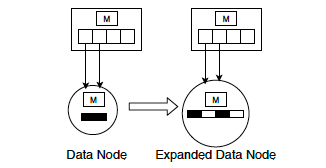
\includegraphics[width=100mm,scale=1]{Figures/alexNodeExpand.png}
    \caption{
     \acrlong{alex} node's expansion machanism.
    }
    \label{fig:alexNodeExpand}
\end{figure}
\subsection{Original Paper on Learned Index}
The \learnindex, a type of learned index structure, was first introduced in the paper titled "The Case for Learned Index Structures" by Tim Kraska \cite{CasedLearnedIndex}. Kraska's proposed method uses machine learning models to structure indexes and demonstrated its feasibility by creating a neural network using Python and TensorFlow. However, the study found that the neural network took $80,000ns$ to execute the model, while a standard B-tree only required $300ns$ for traversal and $900ns$ for the binary search. This discrepancy in execution time highlights the need for further optimization of the \learnindex structure.

Kraska identified three main factors that impact the query performance of the \learnindex. The first is the TensorFlow invocation overhead, which can be reduced through more efficient TensorFlow implementation. The second factor is the challenge of fitting cumulative distribution functions \acrfull{cdf} in neural networks as the \textsf{zoom-out} version may look smooth, but if looked closely, there may be more irregularities in the \acrshort{cdf}. Lastly, the third factor is the high cost of executing complex neural networks, which can be mitigated by using the right techniques.

To address the issue of overhead, Kraska introduced the Learning Index Framework (LIF), which is implemented in C++. LIF allows for the extraction of the neural network's weights and hyperparameters to avoid the framework overhead, thereby reducing the execution time. Additionally, to address the accuracy problem on non-smooth CDFs, Kraska introduced the \acrfull{rmi}. The \acrshort{rmi} is a hierarchical structure of models, where each model takes the key as input and predicts the next model to pick until the final stage, where it predicts the key's position. By using a hierarchical structure of models, \acrshort{rmi} can effectively reduce the number of parameters needed to achieve high accuracy.

Overall, Kraska's study and subsequent research into the \learnindex have demonstrated the potential for machine learning models to improve the performance of index structures. The use of LIF and \acrshort{rmi} has shown promising results in reducing overhead and improving accuracy, respectively. Further research in this area could lead to the development of even more efficient and accurate learned index structures, paving the way for exciting new developments in the field of database management.

\subsection{Static Learned Index}
\acrshort{rmi} is a static \learnindex. It forms a hierachy of models such that the underlying models more accurate representation of the \acrshort{cdf}. Experiments on \acrshort{rmi} shows that it outperforms the B-trees in the index size and the query speed. 

However, one limitation of \acrshort{rmi}, however, is that it only supports read operations. In modern systems, write operations are equally important, and optimizing the performance of both read and write operations is critical for achieving high database performance \cite{lourencco2015no}. Therefore, while the \acrshort{rmi} may offer benefits for read-optimized workloads, it may not be suitable for all applications.

Handling the updates in \acrshort{rmi} is challenging due to the data structure used and the operation is computationally expensive therefore degrading the performnance of the system. The \acrshort{rmi} can perform updates on keys but it has to shift the keys to the right to make space for the new key and also if the position of the keys are slightly modified, it will degrades the model's performance \cite{handlingupdates}. Most of \learnindex require a search within the error bound $\alpha$ to get the exact key position. For example, if \textsf{p} is the position predicted by the machine learning model, then the actual position of the key is within $[p-\alpha,p+\alpha]$. Hence using a binary search with the bounded error, $\alpha$ is guaranteed to get the actual position. Furthermore, re-training is required if there are too many shifts in the element's position or \acrshort{cdf} changes, which is slow when there is a large amount of data in the data structure \cite{ALEX}. 

Hybrid Learned Index (HLI) is another notable static learned index that offers significant performance benefits over traditional indexing structures. HLI is called hybrid because it combines two modules: the Piecewise Linear Approximation Model (PLA) with an error bound and the Rank-Model Index (RMI) without an error bound. The RMI is used to index the PLA-model, with the inner node structure being similar to RMI and ALEX. The leaf node in HLI is the PLA-model with an error bound. The main idea behind HLI is to use RMI to predict the segment that the keys belong to, then traverse until reaching the leaf node, which uses the PLA-model to predict the position.

One significant advantage of HLI is that it outperforms traditional indexing structures. In particular, it achieves up to $4.4\times$ the lookup performance of a B+tree. This performance boost is due to the use of a linear regression model as routing and the prediction only containing multiplication, which is bounded to $O(1)$. HLI also outperforms other learned indexes, such as RMI and PGM index, by about $50\%$.

However, there are some limitations to HLI. One significant drawback is that it does not support update operations such as insertion and deletion. This is because the PLA-model with error bound used in HLI is a static structure that cannot be updated. As a result, HLI is only suitable for scenarios where the data is static and not subject to frequent updates.

In summary, HLI is a static learned index that combines the RMI and PLA-model to achieve significant performance benefits over traditional indexing structures. The use of a linear regression model as routing and the prediction only containing multiplication, which is bounded to $O(1)$, makes HLI an efficient indexing structure. However, the lack of support for update operations limits the applicability of HLI to scenarios where the data is static and not subject to frequent updates.


\subsection{Hybrid Indexes}

In addition to the static learned index, Kraska also introduced the concept of hybrid indexes in his paper \cite{CasedLearnedIndex}. Hybrid indexes are a combination of the learned index and traditional index structures. By using the B-tree as the main index and incorporating the learned index, hybrid indexes aim to leverage the strengths of both methods. This combination can significantly improve the overall operation performance, especially for queries.

The learned index is used to predict the next child node such that it can jump to the next node directly, which improves the traversal process. However, if the distribution of the keys is difficult to learn, then the hybrid index falls back to using the traditional B-tree index. This hybrid approach provides a balance between the accuracy and performance of the index structure.

Moreover, hybrid indexes can benefit from the fact that the learned index can capture the patterns and dependencies among the keys, while the traditional index is efficient in handling updates. This combination provides a robust and flexible approach that can be adapted to different data distributions and scenarios.

The most notable hybrid indexes is called \acrshort{ftingtree} \cite{fittingtree}. The FIT-tree uses B+tree as its index structure. What makes it a learned index is that its leaf nodes contain the linear function to predict the position of the keys. When building the index, \acrshort{ftingtree} divides the keys into several segments, which then it will generate the linear function for each of the segment, which is stored in a B+tree. The key difference between \acrshort{ftingtree} and B+tree is that \acrshort{ftingtree} leaf nodes contain a predictor function while B+tree contains a key. When performing a query, B+tree will have to traverse down until the leaf node finds the particular key. On the other hand, \acrshort{ftingtree}'s leaf node does not contain keys, as it only contains the linear predictor function that represents each segment of the keys. To query in \acrshort{ftingtree}, first, it has to traverse down until the leaf node that represents a particular segment that the key located in. Secondly, it will have to perform a search for the key in the segment within the error bound $pred\_pos \pm err$. The error bound is defined difference between the predicted position and true position of a particular \cite{fittingtree}. 

In \acrshort{ftingtree}, keys are segmented which makes the process of segmenting very important. The algorithm \acrshort{ftingtree} uses is called "\textsf{ShrinkingCone}". It first forms a cone by defining an origin point, high slope ($sl_{high}$) and low slope ($sl_{low}$). The high slope and low slope represent the upper and lower bound of the segment. First the algorithm define $sl_{high} = \infty$ and $sl_{low} = 0$. Then if the key is inside the cone, then the high slope and low slope will be updated by using the key and key's position $\pm$ the \textsf{error}. In addition, the \textsf{ShinkingCone} is a non-optimal algorithm as it does not guarantee that it can produce the most optimal segment. However, there is still an upper bound on the maximum number of segments that the algorithm can produce $min(\frac{|keys|}{2}, \frac{|D|}{error+1})$ and $|D|$ is the number of datasets. This ensures that the amount \acrshort{ftingtree} will not produce more segments than the B+tree that uses a fixed size pages\cite{fittingtree}. 

From the experiment result \cite{fittingtree}, the \acrshort{ftingtree} shows an improvement over index with fixed-size paging in query performance while also memory efficient when compared to full and fixed-size paging index. Eventhough \acrshort{ftingtree} outperforms traditional indexes in lookup and space efficient, there is still some disadvantages of the \acrshort{ftingtree}. Firstly, the performance compared to the other learned index like previously mentioned \acrshort{rmi}. \acrshort{ftingtree} performance gained over B-tree is about $1.5\times$ while \acrshort{rmi} achieve almost $2\times$ the performance of query when compared to B-tree. Secondly, the insertion performance on \acrshort{ftingtree} does not outperform the full B-tree index in the insertion experiment \cite{fittingtree} as \acrshort{ftingtree} requires to perform splitting pages periodically and also performs a segmentation algorithm. 

Apart from \acrshort{ftingtree}, the \textsf{Interpolation-Friendly B-tree} (IFB-tree) is also another hybrid indexes \cite{ifb-tree}. Similar to \acrshort{ftingtree} the IFB-tree also uses B-tree with the node interpolation. The main idea is that node  interpolation is used to estimate the range that the keys located in. For example, if the look up key is $s$, then the interpolated index of $s$ is $\lfloor \frac{s-v_i}{v_{i+1} - v_i} \cdot n \rfloor$ where $v_i$ is the keys before $s$, $v_{i+1}$ is the key after $s$, and $n$ is the node size.

The main advantage of IFB-tree is that it does not consume any extra memory when compared to \acrshort{ftingtree}. \acrshort{ftingtree} requires storing parameters like slope and intercept for the linear regression function. The IFB-tree structure is B-tree which makes it light memory usage when compared to other hybrid indexes. 

However, the main drawback of the IFB-tree is similar to the \acrshort{ftingtree} that its query performs does outperforms a traditional B-tree but does not outperforms \learnindex like \acrshort{rmi}. Based on the result shown by Hadian \cite{ifb-tree}, the result is about up to $1.5\times$ the query performance of traditional B-tree, which is similar while the \acrshort{rmi} is almost $2-3\times$ faster on lookup performance compared to the traditional B-tree. However, if the result is compared to \acrshort{ftingtree}, there is barely any difference in term of lookup performance. The only benefit is that consumes lesser memory than the \acrshort{ftingtree}. 
 
\subsection{Dynamic Learned Index}
The \acrfull{alex} is a dynamic learned index structure proposed by Ding \cite{ALEX} that is designed to support both read and write operations such as insertion and deletion. In terms of structure, \acrshort{alex} is similar to the \acrshort{rmi} as it also has a hierarchy of models. The internal nodes only contain the linear regression model that points to the next child model to predict the partition of the keys. Meanwhile, the leaf nodes contain the keys and records in an array format. However, \acrshort{alex} uses a special data structure called the \textsf{Gapped Array} to store its keys and records in the leaf node.

The \textsf{Gapped Array} is a modified version of an array that leaves gaps between the keys instead of placing the empty spaces at the end of the array. This data structure enables \acrshort{alex} to use model-based insertion, where a model is used to predict the location of the new key, and insert it accordingly.

In addition to model-based insertion, \acrshort{alex} also employs node expansion and retraining to maintain its accuracy. To expand a node, the node must be $80\%$ full before performing the expansion. This criterion is checked when a new key is inserted. Furthermore, \acrshort{alex} performs shifting when a key already exists in the predicted position. It can shift to the right or left, depending on the closest gap.

However, if the distribution of new keys does not follow the existing distribution, the linear regression model becomes inaccurate, leading to a more densely packed region. This can deteriorate the shifting performance, which can take $O(n)$ in the worst case. To solve this issue, \acrshort{alex} requires expanding the data node or retraining the model.

One of the advantages of \acrshort{alex} is its ability to support update operations, which is crucial in real-world systems. This advantage addresses the shortcomings of static learned indexes by using the \textsf{Gapped Array} and model-based insertion.

Furthermore, the use of gaps in the \textsf{Gapped Array} ensures that the average cost of insertion and shifting elements is bounded to $O(\log m)$ instead of $O(m)$ if \acrshort{alex} has to shift keys to the closest gap.

Regarding the query operation, lookup in \acrshort{alex} consists of two stages. First, it traverses down until it reaches the leaf node, which costs $O(\log_m P)$. Secondly, it performs an exponential search as the keys may have shifted around, which costs $O(\log m)$. Since keys can be in any position within the error bound, an exponential search is required. Therefore, the total cost of a query becomes $O(\log_m P + \log m)$.

Overall, \acrshort{alex} is a dynamic learned index that supports both read and write operations with the use of the \textsf{Gapped Array} and model-based insertion. It also employs node expansion and retraining to maintain its accuracy, and its lookup operation has a worst-case time complexity of $O(\log_m P + \log m)$.

Aside from the \acrshort{alex} learned index, the Piecewise Geometric Model index (PGM index) is another dynamic index that aims to support read and write operations \cite{PGM}. The PGM index uses the Piecewise Linear Approximation Model, which segments the keys into multiple linear segments instead of using a machine learning model. This approach is different from \acrshort{ftingtree}, which stores keys in many nodes. However, the PGM index's structure is similar to \acrshort{alex}, with the main difference being in its model.

One of the advantages of PGM index is that it outperforms \acrshort{ftingtree} in terms of operational performance and memory consumption by up to $75\%$. It also dominates \acrshort{rmi} in terms of lookup and space consumption, and it even outperforms the B+tree in terms of space consumption. Moreover, the PGM index has a guaranteed worst-case bound, which is a significant advantage over the static learned index \acrshort{rmi}, as the latter lacks a guaranteed bound. The worst-case time complexity is $O(\log m_{opt} + \log \epsilon)$, and the space complexity is $\Theta(m_{opt})$. Here, $m_{opt}$ refers to the number of $\epsilon$-approximate segments. This makes the PGM index a superior dynamic learned index, as it can adapt based on the keys distribution, which may vary during lookup.

In addition, since the lookup operation is performed frequently in real-world systems, the PGM index's ability to adapt to different distributions during lookup makes it a very notable dynamic learned index. Furthermore, the PGM index also provides a smooth trade-off between operation performance and space consumption, allowing it to scale better in large datasets. In conclusion, the PGM index is a promising dynamic learned index that offers various advantages over other traditional and learned indexes. Future research can explore the PGM index's potential for further optimization and use in various real-world applications. 

RadixSpline is a dynamic learned index introduced by Kipf that uses spline interpolation and a radix table to perform efficient lookup \cite{kipf2020radixspline}. The index consists of two main components: a set of spline points and a radix table. The set of spline points is used to perform spline interpolation for any lookup key, resulting in a predicted position in the array. The radix table is then used to locate the accurate spline point for the queried key.

One of the advantages of RadixSpline is that it only has two hyperparameters to maintain: the number of radix bits $r$ and the spline error $e$. The $r$ parameter determines the size of the radix table and can be adjusted to balance accuracy and memory usage. A larger value of $r$ will increase the size of the radix table exponentially $2^r$, but it will also increase its accuracy.

Another advantage of RadixSpline is that it performs on par with traditional indexes in terms of build time. It is also competitive in terms of lookup performance when compared to other learned indexes. The index is built from the bottom up, constructing the error-bound spline on the keys and then indexing the spline points in the radix table.

However, RadixSpline has a significant drawback in that the radix table size $r$ must be tuned. This can be a challenge as the amount of data grows and the data distribution changes. If the value of $r$ is not carefully chosen, lookup performance can suffer.

Like other learned indexes, RadixSpline provides a good tradeoff between space and time complexity. It requires less space than traditional indexes while achieving comparable lookup performance. The use of spline interpolation also allows it to accurately predict the location of a key in the array, even if the key is not in the set of keys used to construct the index.



\acrfull{lipp} introduced by Jiacheng Wu to support update operations. The primary aim of \acrshort{lipp} is to predict the exact position of a key and eliminate any extra local search required to perform when the model miss predicts the location of the key \cite{LIPP}. The structure of nodes in \acrshort{lipp} is different from other dynamic learned indexes such as the \acrfull{alex}. Unlike the \acrshort{alex}, which has internal nodes and leaf nodes, \acrshort{lipp} only contains the data node, which consists of a gap, a pointer to the child node or a key.

One similarity between \acrshort{lipp} and \acrshort{alex} is that they both use Gapped Arrays in the index structure to reserve gaps for new key insertion. However, during the insertion operation, the main difference is that \acrshort{alex} shifts keys to the closest gaps available, while \acrshort{lipp} creates a new node and replaces the location as a pointer to the new node. The new node will have a gapped array with just two elements. However, the creation of a new node could grow the tree height, making the lookup operation time complexity to be bounded by $O(h)$, where $h$ is the height of the tree.

To solve this problem, \acrshort{lipp} has to perform adjustments (branch pruning) method that helps to reduce the amount of tree height such that it is bounded by the $O(\log N)$. It compares the number of nodes from the previous adjustments, and if it is $2\times$ more nodes than the previous adjustments, then \acrshort{lipp} will trigger the adjustments. Even though the lookup is still bounded by the height of the tree, the adjustment causes the lookup to have a shorter traversal path.

One of the main advantages of the \acrshort{lipp} index is that it outperforms both PGM index and \acrshort{alex} in read and write workloads by $13\times$ and $2.9\times$, respectively. Furthermore, \acrshort{lipp} also outperforms traditional indexes in the read and write operation as well. For the read-only workload, \acrshort{lipp} still outperforms \acrshort{alex}, PGM index, and \acrshort{rmi}. In addition, \acrshort{lipp} eliminates the last mile search completely by using the model to predict the precise position of the queried key.

However, \acrshort{alex} performs better in terms of memory consumption, as it uses gaps to shift the elements, while \acrshort{lipp} consumes extra memory when there is a conflict, as it has to hold two conflicting keys in the leaf nodes. Nonetheless, the \acrshort{lipp} index's benefits make it a promising solution for applications that require both high read and write performance.

In summary, \acrshort{lipp} is a dynamically learned index that uses a unique node structure and adjustments method to provide high read and write performance while eliminating the last mile search completely. Its performance in read and write workloads surpasses that of traditional indexes and other dynamic learned indexes such as \acrshort{alex} and PGM index, making it a promising solution for modern data-driven applications.

Dynamically learned indexes are becoming increasingly popular among researchers. However, these indexes require the presence of empty space, known as gaps, to facilitate the insertion of new elements. This presents a significant challenge in optimizing the algorithms that learn where to place the gaps to improve the efficiency of search and range queries while preserving the sorted order of the data to ensure the correctness of the range query.

However, the success of these methods depends on how well they learn to place the gaps. Poorly placed gaps can negatively impact the search and range query performance, leading to decreased efficiency and degraded accuracy. Therefore, there is a need for machine learning models or algorithms that can effectively learn where to place the gaps to optimize these indexes.


\section{Learned Hash Index}
Hash-table is a fundamental data structure used in many computer science applications, including database management systems. Its primary purpose is to provide an efficient way of looking up data by using a hash function to map keys to positions in an array. However, when two or more keys are mapped to the same position, a conflict occurs, and the hash-table needs to handle it. This is usually done by using a linked list to store all conflicting elements. While Hash-tables are efficient in lookup time, with an average lookup cost of $O(1)$, the worst-case lookup time can be as high as $O(n)$, where $n$ is the number of elements in the linked list.

To reduce the number of conflicts, various techniques have been developed, such as secondary probing or using multiple hash functions, like Cuckoo Hashing. While these techniques reduce the number of conflicts, conflicts can still impact lookup performance and memory consumption.

Kraska introduced the Hash-Model Index, which takes advantage of the underlying data distribution \cite{CasedLearnedIndex}. This index uses a machine learning model to learn the cumulative distribution function (CDF) of the data, providing a better hash function that reduces the number of conflicts by up to $77.5\%$. Unlike tree-based learned indexes, Hash-Model Indexes do not need to maintain sorted order, making them more suitable for supporting updates. When new items are inserted, they are stored in the array or a linked list if there is a conflict.

Hash-Model Indexes provide significant benefits over traditional Hash-tables, improving both lookup performance and memory consumption. Additionally, they provide a scalable solution that can handle large datasets efficiently. However, Hash-Model Indexes require more resources and computational power than traditional Hash tables, making them less suitable for applications with limited resources or computational power. 

\section{Multi-Dimensional Learned Index}
\begin{figure}
    \centering
    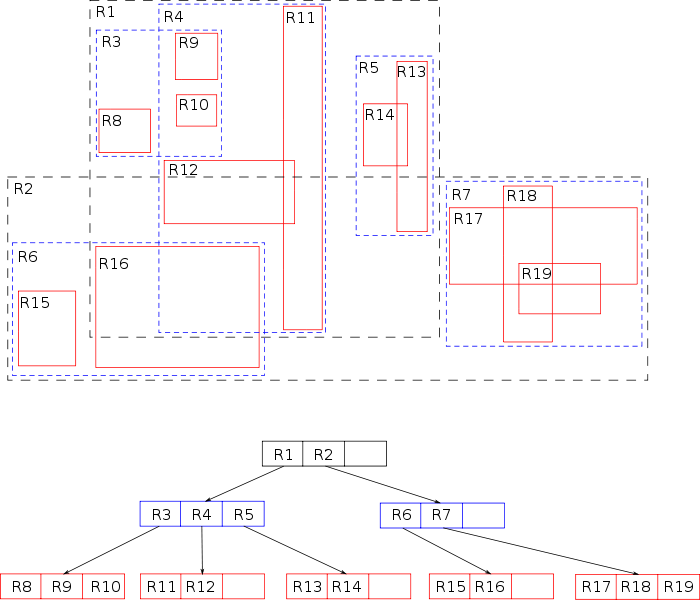
\includegraphics[width=100mm,scale=1]{Figures/R-tree.png}
    \caption{
        R-trees data structure and R-trees' bounding boxes 
    }
    \label{fig:R-tree}
\end{figure}
Scanning and filtering are two typical usages in a database engine \cite{FloodLMD}. To create an order, most database systems use a \btree index on a single attribute. However, when multiple attributes are filtered, using a \btree may lead to latency as the search has to follow pointers and narrow down the search space. To overcome this issue, multi-dimensional indexes with tree-based data structures such as R-trees \cite{r-tree} or k-d trees \cite{kdtree} can be used to improve the scanning performance of queries over multiple columns.

R-trees are a data structure that is commonly used for spatial data \cite{r-tree}. They support multi-dimensional indexing for objects such as geographical coordinates, rectangles, and polygons. R-trees group nearby objects and represent them using rectangular bounding boxes. This helps in reducing the search space during querying, which results in faster query execution times. The R-tree data structure is shown in Figure \ref{fig:R-tree}

In contrast, k-d trees divide the data into subregions using hyperplanes to group nearby points \cite{kdtree}. This approach is commonly used for nearest neighbor search, where the query searches for the data point closest to the given point.

Using multi-dimensional indexes with tree-based data structures provides an efficient solution for querying databases with multiple attributes. These data structures enable faster and more efficient searching by reducing the search space and optimizing the query execution time. As such, they are widely used in database engines for scanning and filtering operations.


Despite the advantages of using multi-dimensional indexes with tree-based data structures, such as R-trees \cite{r-tree} and k-d trees \cite{kdtree}, there are still some limitations that need to be addressed. One such limitation is the difficulty in tuning these indexes, which requires significant engineering efforts. Tuning the index for better performance in one scenario may not necessarily lead to better performance in another scenario \cite{FloodLMD}. Additionally, the indexes cannot adapt to specific workloads and data distributions, which may result in suboptimal performance.

In real-world scenarios, data distribution and query load can vary significantly, making it challenging to design an index that can adapt to changing conditions. Although traditional multi-dimensional indexes like R-trees and k-d trees are commonly used, they have their limitations. In particular, tuning these indexes for optimal performance can be a time-consuming and difficult task that requires significant engineering effort. Moreover, even when these indexes are properly tuned, their performance may not always be optimal, especially when dealing with skewed data distributions or heavy query workloads.

To address these issues, Flood index was developed as an in-memory learned multi-dimensional index that overcomes some of the limitations of traditional indexes \cite{FloodLMD}. Flood index is based on the concept of \acrfull{cdf}, which is used to learn the data distribution and project the multi-dimensional and skewed data into a uniform space. By doing so, the model can predict the data's location and provide fast access to it.

One of the main advantages of Flood index is that it outperforms traditional multi-dimensional indexes like R-trees and k-d trees by eliminating the need for search traversal times. Instead, Flood index relies on machine learning models to predict the location of the data. However, it should be noted that Flood index is designed to work only with read-only workloads. To support the insertion of new data, Flood index can leave gaps similar to \acrshort{alex} or \btree. 

Despite its usefulness, Flood suffers from two major drawbacks: it is not well-equipped to handle a query workload that is skewed \cite{Tsunami}, and it does not maintain uniformly sized grid cells. To address these issues, the Tsunami was developed as an optimized extension of the Flood index \cite{Tsunami}. However, the problem of efficient key insertion persists. One potential solution to this problem is to use gap reservation, which can aid in subsequent key insertions \cite{FloodLMD}.



\section{Learned Bloom Filters}
\begin{figure}
    \centering
    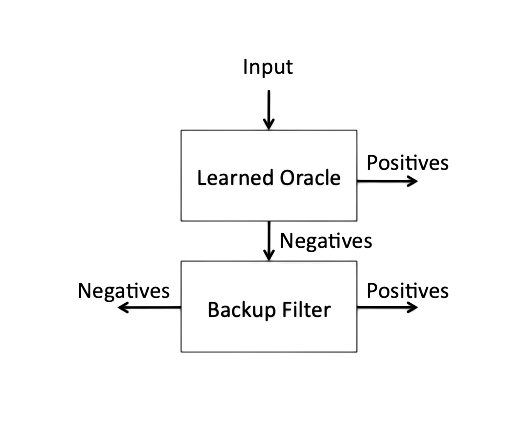
\includegraphics[width=80mm,scale=1]{Figures/learnedBloom.png}
    \caption{
        Learned oracle with backup Bloom filter (backup filter).
    }
    \label{fig:LearnedBloom}
\end{figure}
The Existence index, utilizing a Bloom filter, is one of the most widely used types of indexes in storage systems, databases, and other applications where the fast and efficient determination of set membership is essential. A Bloom filter is a probabilistic data structure that allows for checking if a key is present in a set with an extremely low false negative rate. It does this by utilizing a bit array of size $m$ and $k$ hash functions to map keys to $m$ array positions.

To add an element to the set, the key is inserted into the $k$ hash functions, which returns $k$ different positions in the $m$ array. The bits in these returned positions are then set to $1$, indicating the existence of the corresponding key in the set. During the insertion of a new key, the key is placed into the $k$ hash functions, and the resulting positions in the $m$ array bits are checked to determine if they are all $1$, indicating the presence of the key in the set.

One of the primary advantages of using a Bloom filter is its speed and efficiency in checking for set membership. For instance, Postgres, a popular open-source relational database management system, utilizes a Bloom filter index that allows for the fast exclusion of non-matching tuples \cite{postgresqlBloom}. Bloom filters are also space-efficient as they only require a fixed amount of memory for a given false positive rate.

However, Bloom filters do have a potential drawback, namely the possibility of false positives. A false positive occurs when the filter returns that a key is in the set when it is not. This happens when the hash functions of two different keys result in the same bit positions in the bit array, causing the filter to erroneously report that the key is present. The probability of a false positive is dependent on the size of the bit array $m$, the number of hash functions $k$, and the number of keys inserted into the Bloom filter.

Bloom filters have been found to be highly effective in many applications that require fast and efficient membership checking. However, there are some limitations to traditional Bloom filters, such as their potential for false positives, as discussed earlier. One potential solution to this problem is to augment Bloom filters with machine learning models, as proposed in the Learned Bloom filter \cite{LearnedBloom}.

The Learned Bloom filter is a probabilistic data structure that uses machine learning to make predictions about set membership. However, unlike traditional Bloom filters, the Learned Bloom filter does not provide a zero false negative rate. In other words, there is a chance that the machine learning model will not predict the correct value for a key. To overcome this limitation, the Learned Bloom filter requires a backup Bloom filter that can validate any false predictions made by the machine learning model (as shown in Figure \ref{fig:LearnedBloom}).

It is worth noting that the backup Bloom filter only needs to contain at most $FNR \times n$ elements, where $FNR$ is the false negative rate of the Learned Bloom filter and $n$ is the number of items in the set \cite{LearnedBloom}. This means that if the backup filter contains all the values similar to the traditional filter, it will take up more memory space as it needs to maintain both the backup filter and the Learned Bloom filter. By using this strategy, Bloom filters can potentially save memory space by storing only $n$ bits of elements.

In addition to the Learned Bloom filter, another approach to reducing the false positive rate of Bloom filters is the Sandwich Bloom filter. The Sandwich Bloom filter consists of two layers of Bloom filters, with the Learned Bloom filter sandwiched between them \cite{SandWichBloomFilter}.

The first layer of the Sandwich Bloom filter is the pre-filter, which is a traditional Bloom filter used to eliminate as many false positives as possible before the query reaches the Learned Bloom filter. The pre-filter reduces the workload of the Learned Bloom filter and helps to improve its accuracy. The pre-filter uses a set of independent hash functions to map keys to positions in the bit array, and each position is set to 1. When a key is queried, the pre-filter checks whether all of the corresponding positions in the bit array are set to 1. If any position is not set to 1, the query immediately returns false.

The second layer of the Sandwich Bloom filter is the backup filter, which is a traditional Bloom filter that is used to eliminate false negatives introduced by the Learned Bloom filter. As with the Learned Bloom filter, the backup filter only needs to store at most $FNR \times n$ elements, where $FNR$ is the false negative rate of the Learned Bloom filter and $n$ is the number of items in the set.

By sandwiching the Learned Bloom filter between the pre-filter and the backup filter\cite{SandWichBloomFilter}, the Sandwich Bloom filter can provide high accuracy while minimizing false positives and false negatives. However, like the Learned Bloom filter, the Sandwich Bloom filter is not perfect and may still produce errors. It is important to carefully evaluate the specific requirements of the application before choosing to use a Sandwich Bloom filter.

\section{Data Structure with Gaps}
\begin{figure}
    \centering
    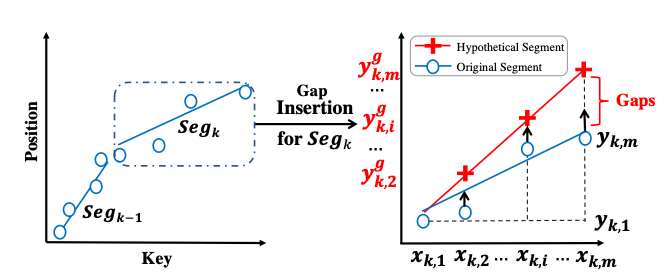
\includegraphics[width=120mm,scale=1]{Figures/gapsinsert.png}
    \caption{
        Gaps Insertion \cite{GapsInsertion}
    }
    \label{fig:gapsinsert}
\end{figure}

The concept of utilizing empty space, also known as gaps, for efficient insertion and deletion operations while maintaining the sorted order of keys is a common approach in various data structures, including the \learnindex\cite{ALEX,LIPP,PGM,fittingtree,FloodLMD,Tsunami, GapsInsertion}. The initial introduction of gaps in data structures can be traced back to \acrshort{alex}, where the \textsf{Gapped Array} technique was introduced. However, since then, several other data structures have utilized the concept of gaps, indicating its importance in designing efficient data structures.

For instance, the ubiquitous B+tree data structure, introduced by Comer in 1979, uses gaps at the end of its leaf nodes to allow for subsequent key insertion without significant overhead \cite{comer1979ubiquitous}. Another example of gap utilization is in the Packed Memory Array, a data structure designed for efficient searching and insertion of elements in compressed arrays, which also employs the use of gaps \cite{PackedMemoryArray}. Similarly, the Packed Memory Quadtree, a variant of the Packed Memory Array designed for two-dimensional spatial data, uses gaps to maintain a balanced tree structure and ensure efficient insertion and deletion operations \cite{packedquadtree}.

Another data structure, the \acrshort{ftingtree}, employs gaps at the end of its array to accommodate new key insertions and deletion operations while still guaranteeing a bounded error in query results \cite{fittingtree}. The \acrshort{ftingtree} shifts keys either left or right, depending on the closest gap, to maintain a balanced tree structure while still achieving optimal query performance.

In addition to reserving space for new data, gapping can also be used strategically to reduce conflicts and improve the efficiency of data structures. For instance, \acrshort{alex} places gaps in a way that reduces the number of conflicts between keys, which in turn minimizes the number of shifts required during insertion. This approach helps to reduce the worst-case shifting time to $O(m)$, where $m$ is the number of keys in the gapped array \cite{ALEX}.

Similarly, the LIPP tree \cite{LIPP} uses gaps to create new child nodes, which can improve the efficiency of the data structure. The PGM-index also uses gaps to reduce the size of its index and improve query times \cite{PGM}. The Tsunami index extends the Flood index by using gaps to maintain uniformly sized grid cells, which in turn improves the query performance \cite{Tsunami}.

Therefore, gapping is a widely used technique in various data structures to ensure efficient insertion and deletion operations while maintaining sorted keys.

\section{A Brief Summary}
The mutable \acrfull{tbli} have been shown to be effective in supporting insert operations while maintaining sorted keys by utilizing gaps. However, as we have observed from previous studies, conflicts arise when space is already occupied, leading to additional computation during insertion operations. To address this challenge, it is crucial to strategically place gaps in the array based on the available information, such as the distribution of existing data. In this project, we aim to minimize the number of conflicts in the \acrshort{lipp} \acrshort{tbli} by leveraging the information about the distribution of existing data, thereby optimizing the insertion overhead caused by conflicts. By strategically placing gaps, we aim to reduce the number of shifts and ensure that the model's error bound is still satisfied, leading to improved performance of TBLIs.

 % Related Work

\lhead{\emph{Preliminary}}
\chapter{Preliminary}
The purpose of this section is to provide an introduction to the concepts and background of our research. By doing so, we hope to provide readers with a better understanding of the context in which our work is situated, and make it easier for them to grasp the key ideas and contributions of our research.

To achieve this goal, we provide an overview of the field of learned indexes and its relevance to data access and manipulation operations and the model used in Learned Index.

In addition, we provide background information on the \acrshort{lipp} approach, which is the foundation of our research. We discuss the structure of \acrshort{lipp}'s node-based index and the components that make it work, such as the gapped array, bitmap index, and linear regression model. We also highlight some of the key features and benefits of \acrshort{lipp}, as well as its limitations.

\section{Linear Regression}
Linear regression is a widely used statistical technique for modeling the relationship between two variables, namely the independent variable, denoted as x, and the dependent variable, denoted as y. The objective of linear regression is to find the best fitting line that represents the relationship between the two variables in the most accurate way possible. The line is represented by the equation $y = mx + c$, where $m$ represents the slope of the line, and $c$ represents the y-intercept.

The main purpose of linear regression is to make predictions based on the relationship between the two variables. In the case of a machine-learned index, linear regression is used to predict the location of the keys in the gapped array. This is done by training a model on a dataset of key and its position. The model learns the relationship between the keys and its location, and can then be used to predict the key's location for new queries.

The process of finding the best fitting line involves minimizing the sum of the squared differences between the actual y-values and the predicted y-values for each data point. This method is known as the method of least squares, and it ensures that the line fits the data points as closely as possible.

One of the reasons why linear regression is used in machine-learned indexes is its simplicity and interpretability. The linear regression model can be easily understood and implemented, and the output can be used to build an index that can efficiently look up rows in the table. Moreover, linear regression can handle large datasets, making it an ideal choice for machine-learned indexes.

In contrast, neural network models can be more complex and computationally expensive, which may cause a large overhead in operations \cite{CasedLearnedIndex}. Therefore, linear regression is a more efficient and practical choice for machine-learned indexes. However, the choice of machine learning algorithm depends on the specific requirements and characteristics of the dataset.

\section{Model-Based Insertion}
\begin{figure}
    \centering
    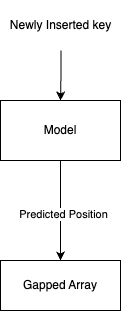
\includegraphics[width=25mm,scale=0.5]{Figures/ModelBasedInsert.png}
    \caption{
     Model-Based Insertion
    }
    \label{fig:model-basedinsertion}
\end{figure}
Model-Based Insertion is essentially an insertion strategy that uses the learned model to determine where newly inserted keys should be placed in the gapped array, previously mentioned in previous section as an array that reserved spaces in between the keys for new insertion, that constitutes the learned index. The algorithm uses the model to predict the location of the new key, and then places it accordingly to ensure that the learned index can efficiently support insert operations. This is achieved by mapping the keys to the linear regression slope of the model, ensuring that the newly inserted keys fit seamlessly within the existing index structure (Figure \ref{fig:model-basedinsertion}).


\acrfull{lipp} adopts a different approach to handling insertion operations compared to other learned indexes such as \acrshort{alex} and PGM \cite{PGM}. Rather than shifting elements or storing them in a temporary buffer to merge later, \acrshort{lipp} employs node creation. This technique involves creating a new node for each new key that is inserted into the index. By creating a new node for each key, \acrshort{lipp} is able to optimize the search operation by ensuring that the output position from the model is exact and precise. This means that \acrshort{lipp} does not need to perform extra searches to locate the key.

However, while \acrshort{lipp}'s node creation approach has several benefits, it also has some limitations. One of the primary concerns with this approach is that it could result in the tree height growing, which could negatively impact the performance of the index. The height of the tree is a critical factor in determining the time complexity of the search operation, and an increase in the height of the tree could result in search operations becoming bound to the height of the tree.
\section{Learned Index Precise Position} \label{LIPP}
\begin{figure}
    \centering
    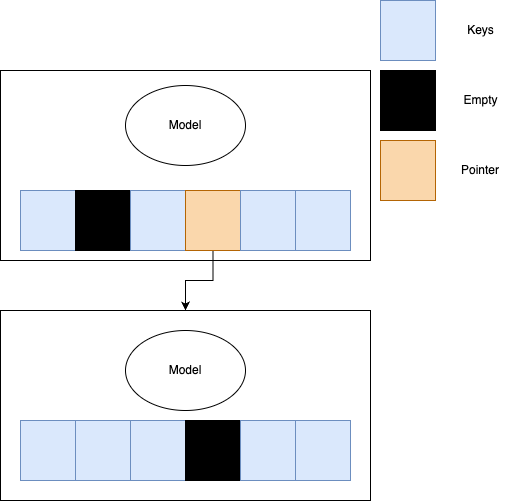
\includegraphics[width=100mm,scale=1]{Figures/LippNode.png}
    \caption{
     \acrshort{lipp} node structure
    }
    \label{fig:lipp-node}
\end{figure}
\acrshort{lipp} achieves prediction precision by using a node-based structure that includes a gapped array, a bitmap index, and a linear regression model (Figure \ref{fig:lipp-node}). These components work together to enable accurate and efficient key access.

Furthermore, \acrshort{lipp} introduces the adjustments or branch pruning to reduce the height of the tree. The conditions to trigger the adjustments are (1) current depth after previous adjustments should not be more than $\beta$ times (set to 2 by default) the previous adjustment, and (2) \conflict number should not exceed $\alpha$ (set to 0.1 by default) from the previous adjustments \cite{LIPP}. 

In this research, we aim to build on the foundations of \acrshort{lipp} by developing an algorithm that further enhances its performance. Our algorithm will focus on optimizing performance of \acrshort{lipp}, specifically by improving the gap placement strategy. By doing so, we aim to improve the accuracy and efficiency of key access operations, enabling faster and more reliable data access and manipulation.
 % Preliminary

\lhead{\emph{Problem Formulation}}
\chapter{Problem Formulation}
\begin{definition}
 (``\emph{Conflict}'') Consider an insertion of a new key to an array stored in a tree node; if the location where the new key should be put in has been occupied, then a \emph{conflict} occurs.
\label{def:conflict}
\end{definition}
\begin{definition}
(``\emph{Gaps}'') Gaps is reserved in the gapped array in between elements to support new keys insertion.  
\label{def:gap}
\end{definition}

\textbf{Where to place gaps such that the Learned Index is efficient to perform operations like insertion, deletion and query ?}
 
 The \acrfull{lipp} tree structure consists of nodes that hold a gapped array, which contains data, pointers to child nodes, and gaps. Gaps are particularly important for \acrfull{tbli} as they enable support for subsequent key insertions and help reduce the number of conflicts and element shifts \cite{ALEX,PGM,fittingtree,LIPP}. \acrshort{tbli} handle conflicts in different ways, with \acrshort{alex} using the shifting method \cite{ALEX} and \acrshort{lipp} creating a new child node \cite{LIPP}. However, while this method ensures that items remain sorted, it comes with the added computational cost of performing shifts or creating a new node during insertion operations. Shifting requires knowledge of the location of the nearest gap to perform the shift, while creating a new node requires following pointers during range queries.

How can we add gaps to a set of keys with increasing positions $\{x, y\}$ in a way that minimizes conflicts while still maintaining or partially maintaining the monotonicity of the key-position relationship? The number of gaps added should be limited to a maximum value of $M$. The distribution of the density of keys in the set, ${X_1, X_2, \cdots, X_n\ | X \in \mathbb{Q}}$, is represented by $Pr[a \leq X_n \leq b]$. The number of gaps inserted between key $X_i$ and $X_{i+1}$ is $m$, and the total number of gaps in the gapped array should not exceed $M$ (i.e., $\sum_{X_1}^{X_n}{m} \leq M$).

One of the main challenges in optimizing the performance of learned indexes is handling dynamic data. When new data is inserted into the data structure, it may follow a different distribution than the existing keys, making it difficult to determine where to insert gaps to minimize conflicts. However, if the newly inserted data follows the same distribution as the existing keys \textbf{static}, the problem becomes simpler to handle. In this case, we can focus on identifying places where the key density is highest and insert gaps accordingly. By doing so, we can reduce the number of conflicts and avoid the need to create new nodes.

On the other hand, for \textbf{dynamic} data, where the distribution of inserted keys may change over time, it is much harder to tackle the problem of minimizing conflicts. In this case, we need to be able to detect slowly changing distributions and adjust the placement of gaps accordingly. This can be achieved by monitoring the distribution of inserted keys and identifying areas where the density has shifted. Once these areas have been identified, we can insert gaps to reduce the number of conflicts.

Reducing the number of conflicts in each node is crucial to ensuring optimal performance of learned indexes. When conflicts occur, we may need to perform extra computations like creating new nodes, which can lead to a larger tree and poor lookup times. Therefore, by minimizing the number of conflicts, we can avoid these extra computations and keep the tree size manageable. Ultimately, this leads to faster lookup times and more efficient use of resources.

Furthermore, expanding gapped arrays and inserting gaps between keys can be a costly operation in terms of retraining the machine learning models used in the indexes. In order to learn the new positions of the keys after gaps have been inserted, the models need to be retrained. However, the amount of time required to retrain the models can vary depending on the complexity of the model used \cite{CasedLearnedIndex}. For instance, a simple linear regression model is used, the retraining process should be fast, as the model only contains multiplications \cite{CasedLearnedIndex,ALEX,LIPP}. However, more complex models, such as neural networks, may take longer to train on larger datasets, making it impractical to retrain the models frequently \cite{CasedLearnedIndex}. Therefore, finding a balance between the complexity of the model and the time required to retrain it is essential when optimizing dynamic learned indexes. 



The current state-of-the-art dynamic \learnindex, \acrshort{lipp}, supports updates by optimizing the keys to fit a linear model. This ensures that the model always predicts the correct position of the keys. However,  \acrshort{lipp} creates a new node for each update, which can make operations like insertion and deletion bounded by the height of the tree.

The goal of this thesis is to design a dynamic \learnindex that supports updates and performs better than \acrshort{lipp} in terms of insertion and deletion time. To do this, we optimize the placement of gaps in the learnindex. This allows the \learnindex to adapt to the distribution of keys and place gaps in densely packed areas, which reduce the number of new child nodes that need to be created.



 % Problem Formulation

\lhead{\emph{Methodology}}

\chapter{Methodology} \label{implementation}
The use of gaps in \acrshort{lipp} trees is crucial for supporting subsequent key insertions and reducing the number of shifts and conflicts that occur during insertion operations. However, the handling of conflicts in \acrshort{lipp}  trees differs from other tree structures like \acrshort{alex}. While \acrshort{alex} uses the shifting method to handle conflicts, \acrshort{lipp}  trees create a new child node. This method guarantees that items remain sorted, but it introduces extra computation cost during insertion operations.

The objective of this study is to explore methods of optimizing mutable tree-based \learnindex by strategically creating gaps for future insertions to minimize conflicts. This approach differs from \acrshort{fmcd} \cite{LIPP}. The study investigates two initial implementations: (1) Histogram, and (2) Partially sorted insertion strategy.

Our first implementation, Histogram, involves creating a histogram of the dataset to determine the frequency distribution of the keys. Based on this distribution, our algorithm leaves gaps in the appropriate places to accommodate future insertions, thereby reducing the number of conflicts that occur during insertion.

Our second implementation, Insert strategy partial sorted, focuses on identifying the most suitable location to insert a new key based on available space after the predicted position. The algorithm examines the dataset and creates a partially sorted list, which contains the keys in ascending order up to a certain point, and then the rest of the keys are left unsorted. This approach allows for more efficient insertion by taking advantage of the sorted section of the list while still leaving room for new keys to be inserted without causing conflicts.

\section{Histogram}
Histogram is a sequence of bin and bin is a partition of a range of keys which represents the distribution of the keys in the node.
Maintaining a histogram in each node of the \acrshort{lipp} tree structure is a powerful method for optimizing the placement of gaps in the array. \acrshort{lipp} triggers rebuilding of tree nodes when the node's depth is two times. We use histogram to approximate the distribution of the items in the gapped array and insert gaps based on the distribution and then train the model based on the the keys' position. 

However, the success of this method depends on selecting an appropriate bin size for the histogram. The challenge is to strike a balance between the overfitting and underfitting of the data in the histogram. Overfitting occurs when the bin size is too small, which leads to too many bins and lack of generalization to unseen data. Underfitting occurs when the bin size is too large, which leads to fewer bins and a loss of detail in the data.

There are several methods for selecting an appropriate bin size for the histogram, including the \acrfull{fdrule} and Sturges' rule \cite{sahann2021histogram}. For our histogram algorithm, we use Freedman-Diaconis rule to attain the bin width for the histogram.
Each nodes has its own bin width to reflect on the data in its gapped array and its subtree. 

The Freedman-Diaconis rule is a method for determining an appropriate bin width for creating a histogram. Histogram is useful for visualizing the distribution of a dataset. They work by dividing the range of data into a series of bins and counting the number of data points that fall into each bin. 

In addition, the bin width is an important parameter in constructing a histogram, as it determines the number of bins and the level of detail displayed in the frequencies of the keys. If the bin width is too small, the histogram may show too much detail and become difficult to read. If the bin width is too large, the histogram may lose important information and become overly simplified.

\begin{equation}\label{eq:IQR}
    IQR = Q_3 - Q_1
\end{equation}


The Freedman-Diaconis rule aims to find an appropriate bin width that balances these trade-offs. It is based on the \acrfull{iqr} of the data (Equation \ref{eq:IQR}), which is a measure of the spread of the data that is less sensitive to outliers than the range or standard deviation. The \acrshort{iqr} is calculated by subtracting the value at the 25th percentile $(Q_1)$ from the value at the 75th percentile $(Q_3)$. It represents the range of the middle 50\% of the data.

\begin{equation}\label{eq:FreedmanDiaconis}
    Bin Width = \frac{c\times IQR}{\sqrt[3]{n}}
\end{equation}

The rule then calculates an "optimal" bin width as the product of a constant factor (usually set to 1.0) and the \acrshort{iqr}, divided by the cube root of the number of data points (Equation \ref{eq:FreedmanDiaconis}). This formula scales the bin width with the sample size, so that the bin size becomes smaller as the sample size increases. The cube root is used to find a balance between having too few bins and too many bins.

The Freedman-Diaconis rule is particularly useful for datasets that have a skewed or multimodal distribution. These types of datasets can be difficult to visualize accurately with histograms using other methods. The rule adjusts the bin width to account for the spread of the data in the middle 50\% of the distribution, rather than just the range of the data. 

While our approach of using a histogram to analyze the distribution of collected data and selecting an optimal bin width has several advantages, it is important to note that there are certain limitations to this technique. One of the primary drawbacks is that it may not perform well on real-world datasets where the distribution of the data is random and does not follow a specific pattern or distribution.

In such cases, a histogram-based approach may not be as effective, as the data may be too complex and varied to be analyzed using a simple histogram. This may result in suboptimal bin width selection, which in turn can lead to less efficient adjustments to the \learnindex structure.



\section{Partial Sorted Array} \label{partialsorted}
To address extra computation issue, we propose another method that uses of a partially sorted array in \acrshort{lipp} trees \cite{partialMonotonic}. A partially sorted array allows the algorithm to continue the search for the correct position of a new key forward until it reaches a specified limit. For example, when inserting a key $1.2$ into the gapped array $[1,2, GAP,3]$, the algorithm would ideally insert the key between one and two to maintain sorting. However, with partial sorting, the algorithm continues searching until it hits the limit $key+\epsilon$, where $\epsilon$ is a pre-defined limit. In this case, the algorithm scans forward until it reaches the number that is not more than three.

Partial sorting reduces the number of conflicts during insertion operations, but it does not completely eliminate them. Partially sorted arrays delay conflicts for future insertions, meaning conflicts will eventually occur when the available space runs out. For example, if the array is $[1,2,1.2,3,4, GAP]$ and the key $2.4$ is inserted, the algorithm must search beyond $4$ to find the gap. To address this issue, a limit $\epsilon$ is introduced to specify the amount of space to scan after the actual position where the insertion is intended. If space is exhausted after $key + \epsilon$, a new child node is created to hold the remaining keys.

When performing a range query on a partially sorted array, the algorithm does not scan from the beginning to the end of the range. Instead, it scans forward until it reaches the limit specified during the insertion operation to ensure the correctness of the range query. The use of partially sorted arrays in \acrshort{lipp} trees aims to amortize the cost of slow insertion, where the algorithm has to scan until it reaches the $key+\epsilon$ limit, with fast insertion where there is still space available.




% \begin{figure}
%     \centering
%     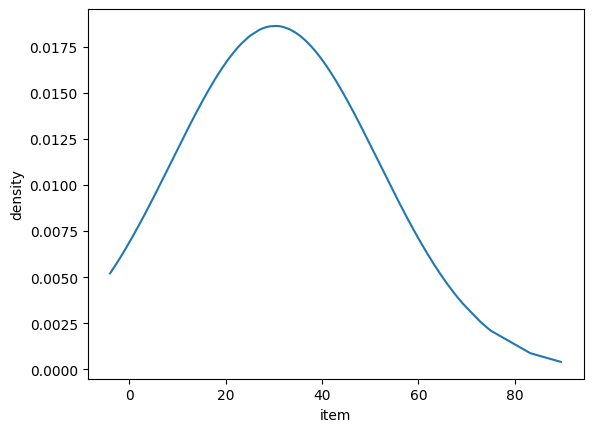
\includegraphics[width=80mm,scale=1]{Figures/normaldist.png}
%     \caption{
%         Normal distribution of Synthetic dataset
%     }
%     \label{fig:NormalDist}
% \end{figure}

% \subsubsection{Histogram}
% \begin{figure}
%     \centering
%     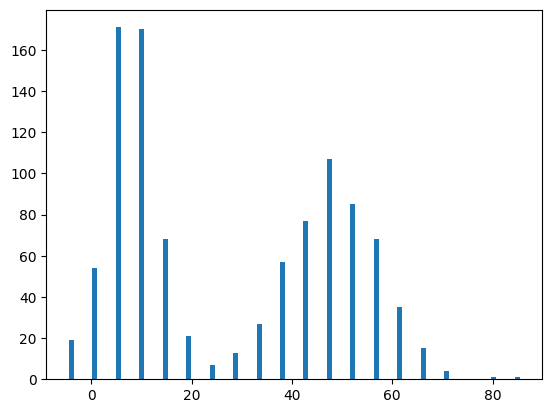
\includegraphics[width=80mm,scale=1]{Figures/histogram.png}
%     \caption{
%         Histogram of Synthetic data
%     }
%     \label{fig:Histogram}
% \end{figure}

% \subsubsection{Insert strategy Partial Sorted}





 % Methodology

\lhead{\emph{Histogram}}
\chapter{Histogram}

In this section, we will delve into the implementation details of histograms and explore various operations such as insertion, update, and deletion. Understanding these fundamental aspects will provide you with a comprehensive understanding of how histograms are built and manipulated.

\section{Implementation Details}
\subsection{The Insertion Algorithm}


\begin{figure}[H]
    \centering
    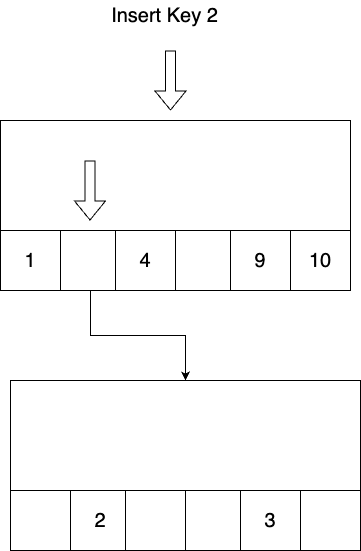
\includegraphics[width=50mm,scale=1]{Figures/InsertionHist.png}
    \caption{
     Example of Histogram Insertion
    }
    \label{fig:HistInsertionExample}
\end{figure}

The strategy we employ for the insertion of histograms is very similar to that of the baseline strategy. However, there are some noteworthy differences in the way we rebuild nodes. Rather than relying on the traditional methods, we use a histogram approach to obtain an approximate distribution of the data. This allows us to generate keys, denoted by $x$, and their corresponding positions or labels, denoted by $y$.

To further refine the model, we use Ordinary Least Square (OLS) to obtain the slope and y-intercept for linear regression. This aids in the accurate identification of conflicts within the data. The rebuilding process occurs when a new node has a depth that is at least twice that of the previous node, in a similar fashion to the baseline strategy.
\begin{algorithm}
\caption{Histogram Insertion}
\begin{algorithmic}[1]

\Procedure{insert}{node, key}
\State $current\_node \gets node$
\State $path\_size[]$
\While{$node \neq null$}
\State $pos \gets PREDICT\_POS(current\_node, key)$
\If{$pos$ is child node}
    \State $current node \gets node[pos]$
    \State $path\_size[i] \gets node$
\Else
    \State $key\_pos = PREDICT\_POS(current\_node, key)$
    \State $node[key\_pos] \gets key$
    \State update $frequency\_array$
\EndIf
\EndWhile
\For{$i \gets 0$ to $path\_size - 1$}
   \State $node \gets path[i]$
    \If{rebuilding criteria}
        \State $keys \gets collect\_keys$
        \State $new\_node \gets rebuild\_tree$
        \State $path\_size[i] \gets new\_node$
    \EndIf
\EndFor

\EndProcedure
\end{algorithmic}
\end{algorithm}

In cases where conflicting elements arise, a new node is created to ensure the integrity of the data. However, the creation of new nodes comes with an additional computation, which slows down the insertion time. This is because the model needs to be trained to accommodate these conflicting keys and accurately insert them into the gapped array.

As an example in Figure \ref{fig:HistInsertionExample}, if a key $2$ is inserted into an existing tree, the predicted position will be $1$. However, $1$ is already occupied, so the tree will create a new node that contains $2, 3$ and replace the root node $pos[1]$ as the pointer pointing to the child node.

Overall, the insertion strategy for histograms relies on a combination of techniques such as the use of OLS and histogram analysis to ensure that the data is accurately represented and conflicts are resolved promptly. While it may result in slightly slower insertion times, the benefits of a more accurate representation of the data outweigh the costs.

\subsection{The Query Algorithm}

\begin{figure}[H]
    \centering
    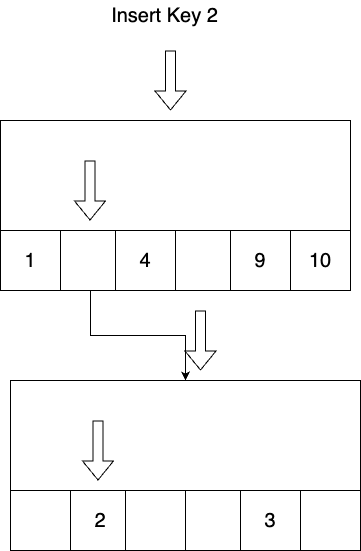
\includegraphics[width=70mm,scale=1]{Figures/QueryHist.png}
    \caption{
     Example of Histogram Query
    }
    \label{fig:HistQueryExample}
\end{figure}
To perform a search operation in \learnindex, the algorithm starts at the root node of the tree and traverses down to the leaf nodes to find the data. One of the advantages of \learnindex is that it uses a model-based insertion technique, which allows it to perform search operations efficiently. When there is a conflict during insertion, \learnindex creates a new child node rather than shifting the keys to the closest gaps. This ensures that there are no misplacement in the index, which can slow down search operations by making performing a search after traversing down the tree.

The search algorithm in \learnindex starts by pushing the root node into the stack. Using the current node's linear regression model, the algorithm predicts the position of the keys it is searching for. It then checks if the predicted position is a child or a key. If the predicted position is a child, the algorithm pushes the child node onto the stack and continues the search. If the predicted position is a key, the algorithm returns the key.
\begin{algorithm}
\caption{Histogram Query}
\begin{algorithmic}[1]
\Procedure{query}{node, key}
\State $current\_node \gets node$
\While{$node \neq null$}
\State $pos \gets PREDICT\_POS(current\_node, key)$
\If{$pos$ is child node}
    \State $current node \gets node[pos]$
    
\Else
    \State $key\_pos = PREDICT\_POS(current\_node, key)$
    \State \Return $node[key\_pos]$
\EndIf
\EndWhile
\State return null
\EndProcedure
\end{algorithmic}
\end{algorithm}

The child node continues to be pushed onto the stack until the algorithm reaches the node that contains the key it is searching for. This process allows for efficient search operations, as the algorithm only explores the parts of the tree that contain the key it is searching for.

As an example, in Figure \ref{fig:HistQueryExample}, if we perform a query after the insertion for a key $2$, the model predicts the location of key $2$ in location $1$ and it has to follow the pointer down to leaf node and use the model at leaf node to predict the location of key $2$.
\subsection{The Deletion Algorithm}


\begin{figure}[H]
    \centering
    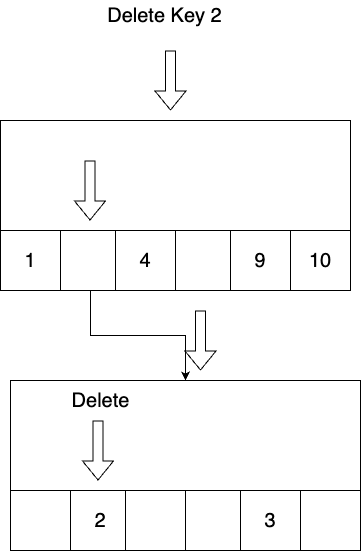
\includegraphics[width=70mm,scale=1]{Figures/DeleteHist.png}
    \caption{
     Example of Histogram Delete
    }
    \label{fig:HistDeleteExample}
\end{figure}
Deletion is an essential operation for any data structure that stores data, and \learnindex is no exception. Deletion in \learnindex follows a similar strategy as search, where the algorithm has to traverse down the tree until reaching the node where the key is located. Once the node is found, the key can be removed from the tree.
However, there is a critical difference between deletion and search in \learnindex. During deletion, the algorithm must also free up space in the gapped array, and also update the bitmap index that this position contains a gap instead of a key.

\begin{algorithm}
\caption{Histogram Delete}
\begin{algorithmic}[1]

% \State $\texttt{MAX_DEPTH} \gets 128$
\Procedure{Delete}{node, key}
\State $current\_node \gets node$
\While{$node \neq null$}
\State $pos \gets PREDICT\_POS(current\_node, key)$
\If{$pos$ is child node}
    \State $current node \gets node[pos]$
    
\Else
    \State $key\_pos = PREDICT\_POS(current\_node, key)$
    \State delete $node[key\_pos]$
    \State update $frequency\_array$
\EndIf
\EndWhile
\EndProcedure
\end{algorithmic}
\end{algorithm}
To perform the deletion, the algorithm starts at the root node and uses the same model-based approach to predict the position of the key. As the algorithm descends the tree, it checks each node's bitmap to determine whether the key is present in that node. Once the node containing the key is found, the key is deleted, and the algorithm updates the bitmap that stores it in the current node.

For an example Figure \ref{fig:HistDeleteExample}, deleting key $2$ requires traversing down from root node until reaching key $2$ nodes similar to query, then use the model to predict the location of key $2$ before deleting it from the gapped array.  

\subsection{The Range Query Algorithm}
\begin{algorithm}
\caption{Histogram Range Query}
\begin{algorithmic}[1]

\Procedure{range\_query}{root, lower, upper}
  \State $stack \gets \text{empty stack}$
  \State $current\_node \gets root$
  \State $keys \gets \text{empty array}$
  \While{$current\_node \neq \text{null}$ \textbf{ or } $stack$ is not empty}
    \While{$current\_node \neq \text{null}$}
      \State $\text{push } current\_node \text{ to } stack$
      \State $pos \gets \text{PREDICT\_POS}(current\_node, \text{lower})$
      \If{$pos$ is a child node}
        \State $current\_node \gets current\_node[pos]$
      \Else
        \State \textbf{break}
      \EndIf
    \EndWhile
    \If{$\text{stack}$ is not empty}
      \State $current\_node \gets \text{pop a node from } stack$
      \State $key\_pos \gets \text{PREDICT\_POS}(current\_node, \text{lower})$
      \For{$i \gets \text{key\_pos}$ to $\text{node\_size}-1$}
        \If{$\text{node}[i] \leq \text{upper}$}
          \State $\text{append } \text{node}[i] \text{ to } keys$
        \Else
          \State \textbf{break}
        \EndIf
      \EndFor
      \State $current\_node \gets current\_node[\text{next position}]$
    \EndIf
  \EndWhile
  \State \textbf{return} $keys$
\EndProcedure
\end{algorithmic}
\end{algorithm}

Range queries are an essential operation in \learnindex, particularly when dealing with sorted collections of keys. Such queries involve searching for a range of keys within a given dataset and are commonly used in a wide range of applications, including databases, search engines, and information retrieval systems.

One of the advantages of using a sorted dataset is that it makes range queries relatively easy to perform. By searching for the first key in the range and then iterating through the data structure to collect all keys until the end key is reached, the algorithm can efficiently retrieve all of the data within the specified range.


\subsection{The Adjustments Algorithm}

\begin{algorithm}
\caption{Histogram Gap Distribution}
\begin{algorithmic}[1]
\Procedure{Histogram Distribute}{node, keys, size, gap\_multiples}
 \State $\text{num\_bins} \gets 0$
  \State $\text{bin\_size, bin\_width} \gets node.hist$
  
  \State $\text{total\_gaps} \gets \text{round}(size \times \text{gap\_multiples})$
  
  \State $\text{gaps\_per\_bin} \gets \text{empty vector}$
  \State $\text{sum\_counts} \gets 0$
  
  \For{$i \gets 0$ to $\text{num\_bins} - 1$}
    \State $\text{gaps} \gets \text{round}(bin\_size \times \text{total\_gaps} / size)$
    \State $\text{gaps\_per\_bin}.\text{push\_back}(\text{gaps})$
    \State $\text{sum\_counts} \gets \text{sum\_counts} + bin\_size$
  \EndFor
  
  \State $\text{result} \gets \text{empty array of size} \ 2 \times size$
  \State $\text{min\_val} \gets \text{keys}[0]$
  \State $\text{outSize} \gets 0$
  
  \For{$i \gets 0$ to $size - 1$}
    \State $\text{bin\_index} \gets \text{floor}((\text{keys}[i] - \text{min\_val}) / \text{bin\_width}$
    
    \State $\text{result}[\text{outSize}] \gets \text{keys}[i]$
    \State $\text{outSize} \gets \text{outSize} + 1$
    
    \If{$\text{hist.first}[\text{bin\_index}] > 0$}
      \State $\text{result}[\text{outSize}] \gets 0$
      \State $\text{hist.first}[\text{bin\_index}] \gets \text{hist.first}[\text{bin\_index}] - 1$
      \State $\text{outSize} \gets \text{outSize} + 1$
    \EndIf
  \EndFor
  
  \State \textbf{return} \text{result}
\EndProcedure
\end{algorithmic}
\end{algorithm}
The strategy we employ to make adjustments to the \learnindex structure utilizes the same condition as \acrshort{lipp}. Prior to making any adjustments, our algorithm traverses the data structure and collects the keys that will be involved in the adjustments. We then create a new node to store these keys. 

However, our approach differs in the way we analyze the collected data. Rather than using \acrfull{fmcd}\cite{LIPP}, we use a histogram to examine the distribution of the data and select a bin width based on the characteristics of the collected data.  By doing so, we are able to make more informed decisions about the optimal size of the bin width, which can ultimately lead to more efficient and effective adjustments to the \learnindex.




\section{Theoretical Analysis}
When inserting a node into a gapped array, the algorithm must traverse down the tree until it finds an empty gap to fill. This process takes $O(\log N)$ time.

However, the linear regression model used to predict the position of keys is much more efficient, taking only $O(1)$ time due to its reliance on simple multiplication operations. Additionally, when a new node is inserted into the tree, the histogram in each node must be updated to reflect the new frequency of data points.

To accomplish this, we use an array of frequencies and calculate the bin index using the formula $bin\_index = floor((data\_point - min\_value) / bin\_width)$. The calculation of the bin index for a single data point takes only $O(1)$ time due to the simplicity of the arithmetic operations and the use of the floor function. However, insertions need to be readjusted when the condition is met, similar to the \acrshort{lipp} index, which will cost $O(N\log N)$ where N is the number of keys in the tree. In adjustments, gap redistribution is required and retrained the model to get the accurate prediction of keys and location. However, the adjustments do not occur every time we traverse down the tree path. In this case, we can amortize the cost such that we save $\log N$ credit every time we pass a path which makes the insertion costs similar to the baseline, which is $O(\log^2 N)$

However, the time complexity for updating the histogram frequency with bin width using an array varies depending on the number of data points that map to the same bin. In the best case, the time complexity for updating the frequency is $O(1)$, as updating an element in an array takes constant time. However, in the worst case, the time complexity for accessing the frequency element is $O(\epsilon)$, where $\epsilon$ is the number of data points that map to the same bin. This is because computing the index to access the array element can require linear time.

Therefore, the efficiency of updating the histogram frequency in each node during the insertion process can vary greatly depending on the number of data points that map to each bin. However, the overall time complexity of inserting a new node into the gapped array is dominated by the traversal down the tree, which takes $O(\log N)$ time.

However, deleting a key in the \learnindex algorithm involves more than just traversing down the tree. Once the key is located, the algorithm needs to perform deletion and free the memory in the gapped array that was allocated for the key being deleted. This can be a more complex process than insertion, which only involves finding an empty gap in the gapped array and filling it with a new key.

Similar to insertion, when deleting a key, the algorithm must traverse down the tree until it reaches the appropriate node. This process takes $O(\log N)$ time, where $N$ is the number of elements in the tree. Once the node is reached, the algorithm must search for the key to be deleted. If the key is found, the algorithm must then perform deletion and free up the memory in the gapped array for future key insertion. In addition, it takes the same time complexity to update the histogram.

Querying a key in the \learnindex algorithm involves traversing down the tree until the model predicts that the key is located at the current node. This process takes $O(\log N)$ time, where $N$ is the tree's height. Once the key is found, the algorithm returns its position in the gapped array.

The time complexity for querying a key in the \learnindex algorithm is dominated by the traversal down the tree. Since the linear regression model used by the algorithm can accurately predict the position of keys, the search process is generally efficient and does not require additional time complexity.

In summary, the \learnindex algorithm is designed to provide efficient querying capabilities with time complexity of $O(\log N)$, where $N$ is the number of elements. 


 % Histogram 

\lhead{\emph{Partial Sorted Insert Strategy}}
\chapter{Partial Sorted Insert Strategy}
In this section, we will delve into the implementation details of partial sorted insertion strategy and explore various operations such as insertion, update, and deletion. Understanding these fundamental aspects will provide a comprehensive understanding of how partially sorted handles new key insertion.
\section{Implementation Details}

\subsection{The Insertion Algorithm}




\begin{figure}[H]
    \centering
    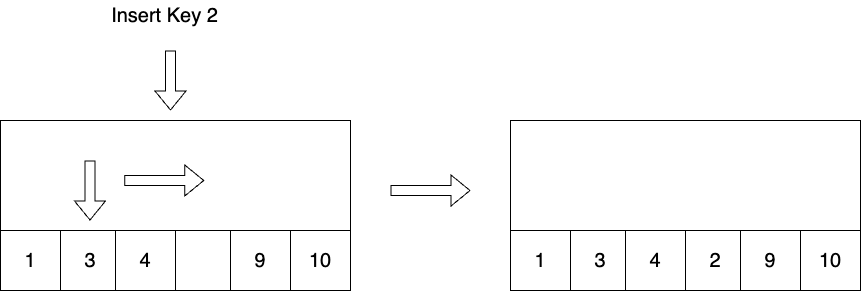
\includegraphics[width=120mm,scale=1]{Figures/PartialSortedInsertion.png}
    \caption{
     Example of Partially Sorted Insertion Strategy
    }
    \label{fig:PartialInsertionExample}
\end{figure}

When it comes to inserting a new key in the partially sorted gapped array of the \acrshort{lipp} index, the process differs from that of a fully sorted array. Instead of creating a new node in the tree for the key, the algorithm must search for the next available gap within the specified limit to insert the new key. This approach is designed to reduce the memory overhead of the \learnindex data structure, as it eliminates the need to create new nodes for every new key.

Specifically, the algorithm traverses down the tree until it reaches a node containing a key that is within the predicted position of the new key. Once such a node is found, the algorithm scans forward within the array for the next available gap to insert the new key. This process ensures that the new key is inserted in the correct position in the partially sorted array, without requiring the creation of new nodes in the tree.
\begin{algorithm}
\caption{Partially Sorted Insertion Strategy}
\begin{algorithmic}[1]

% \State $\texttt{MAX_DEPTH} \gets 128$
\Procedure{insert}{node, key}
\State $current\_node \gets node$
\State $path\_size[]$
\While{$node \neq null$}
\State $pos \gets PREDICT\_POS(current\_node, key)$
\If{$pos$ is child node}
    \State $current node \gets node[pos]$
    \State $path\_size[i] \gets node$
\Else
    \State $key\_pos = PREDICT\_POS(current\_node, key)$
    \If{$node[key\_pos]$ is not empty} 
        \State $key\_pos \gets search\_next\_\epsilon(key\_pos)$
    \EndIf
    $node[key\_pos] \gets key $
    % \State update $frequency\_array$
\EndIf
\EndWhile
\For{$i \gets 0$ to $path\_size - 1$}
   \State $node \gets path[i]$
    \If{rebuilding criteria}
        \State $keys \gets collect\_keys$
        \State $new\_node \gets rebuild\_tree$
        \State $path\_size[i] \gets new\_node$
    \EndIf
\EndFor

\EndProcedure
\end{algorithmic}
\end{algorithm}
However, this approach does have a potential downside in terms of computational overhead. Since the partially sorted array is not fully ordered, the algorithm may need to search further than it would in a fully sorted array to find an available gap to insert the key. This extra search can add additional computational complexity to the insertion process, as the algorithm must spend more time searching for an available gap in the array.

To handle conflicts, partially sorted \learnindex needs to iterate $\epsilon$ spaces after predicted position to collect all the partially sorted keys. This process can be time-consuming, especially if the data set is large. In some cases, the algorithm may need to rebuild the whole node entirely to properly sort the partially sorted keys. As seen from the example Figure \ref{fig:PartialInsertionExample}, if a key $2$ is inserted into an existing tree, it will search for an empty space after the predicted position $1$ and insert the key into the empty location. However, it will only search for $\epsilon$ amount of spaces.

A specific example of this can be seen in the context of a gapped array. When the predicted position contains a partially sorted keys, this requires the algorithm to recursive rebuild of both keys. In such cases, the algorithm needs to iterate through the gapped array to collect all the partially sorted keys that may be located $\epsilon$ distance away from the predicted position.

Moreover, rebuilding the gapped array becomes necessary if the predicted position is itself a partially sorted key. In this scenario, a recursive rebuilding process must be undertaken to ensure that the gapped array is correctly sorted, which will also affect the running time of this algorithm.

As mentioned earlier, one approach to handling conflicts in a gapped array data structure is to use a recursive rebuilding approach. However, an alternative approach is to use the percentage of partially sorted keys to determine whether to rebuild the whole node.

This approach takes advantage of the fact that when a high percentage of the keys in a gapped array is partially sorted, it may be more efficient to rebuild the whole node rather than to attempt to rebuild when the \conflict happens. If the number of partially sorted keys is more than $\frac{1}{2}$ of the number of gapped array lengths, then rebuilding the whole node should be considered.

However, it is essential to note that this approach has limitations and may not always be the most efficient way to handle conflicts in a gapped array. It is also essential to consider other factors, such as the size of the data set and the computational resources available.

In this particular work, we will only be tested on the recursive rebuilding approach. This decision was likely made to simplify the testing process and to provide a clear comparison between baseline and partially sorted gapped array. 


\subsection{The Query Algorithm}

\begin{figure}[H]
    \centering
    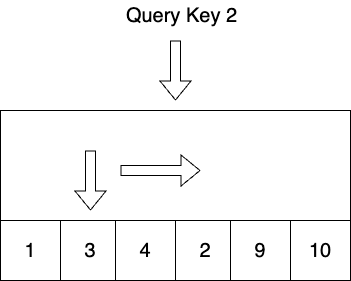
\includegraphics[width=70mm,scale=1]{Figures/QueryPartial.png}
    \caption{
     Example of Partially Sorted Query
    }
    \label{fig:PartialQueryExample}
\end{figure}
When it comes to querying a key in the partially sorted gapped array of the \learnindex algorithm, the process is similar to that of insertion. Like insertion, the algorithm must traverse down the tree until it reaches a node containing a key that is within the predicted position of the queried key. If the key in the node is not the same as the queried key, the algorithm must then scan forward within the array up to the specified limit.

This approach efficiently locates the queried key within the partially sorted array while minimizing the memory overhead of the \learnindex data structure. By accurately predicting the position of the queried key using the linear regression model, the algorithm can quickly navigate the gapped array and locate the keys within the partially sorted limit.
\begin{algorithm}
\caption{Partially Sorted Query}
\begin{algorithmic}[1]
\Procedure{query}{node, key}
\State $current\_node \gets node$
\While{$node \neq null$}
\State $pos \gets PREDICT\_POS(current\_node, key)$
\If{$pos$ is child node}
    \State $current node \gets node[pos]$
    
\Else
    \State $key\_pos = PREDICT\_POS(current\_node, key)$
    \If{$key\_pos \neq key$}
        \State $key\_pos \gets search\_next\_epsilon(current node, key)$
    \EndIf
    \State \Return $node[key\_pos]$
\EndIf
\EndWhile
\State return null
\EndProcedure
\end{algorithmic}
\end{algorithm}
However, scanning forward in the array can potentially add computational complexity to the querying process, mainly if the limit specified is far from the predicted position of the queried key. The algorithm must search through the array to find the next available gap within the limit, which can result in additional computational overhead. 

As an example in Figure \ref{fig:PartialQueryExample}, if searching for $2$, which is a partially sorted key, the predicted position by the model will be the same as insertion, which is $pos \gets 1$. However, the algorithm must perform a sequential search for $\epsilon$ spaces after the predicted position to get key $2$.


\subsection{The Deletion Algorithm}

\begin{figure}[H]
    \centering
    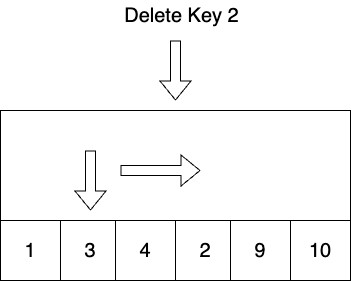
\includegraphics[width=70mm,scale=1]{Figures/PartialSortedDelete.png}
    \caption{
     Example of Partially Sorted Delete
    }
    \label{fig:PartialSortedDeleteExample}
\end{figure}
When it comes to deletion in a data structure such as a \learnindex, the process typically involves searching for specific keys that need removal. However, in the case of a partially sorted gapped array structure, this search process can be more complex, as the keys are not necessarily contiguous and may be spread out over multiple sections of the array.

To perform deletion efficiently in a partially sorted gapped array, the \learnindex algorithm must continue searching for the target keys beyond the predicted location. This typically involves searching until the $\epsilon$ partial sorted limit, where $\epsilon$ is the number of empty spaces after the predicted position the keys can be inserted into.
\begin{algorithm}
\caption{Partially Sorted Delete}
\begin{algorithmic}[1]
\Procedure{delete}{node, key}
\State $current\_node \gets node$
\While{$node \neq null$}
\State $pos \gets PREDICT\_POS(current\_node, key)$
\If{$pos$ is child node}
    \State $current node \gets node[pos]$
    
\Else
    \State $key\_pos = PREDICT\_POS(current\_node, key)$
    \If{$key\_pos \neq key$}
        \State $key\_pos \gets search\_next\_epsilon(current node, key)$
    \EndIf
    \State delete $node[key\_pos]$
\EndIf
\EndWhile
\EndProcedure
\end{algorithmic}
\end{algorithm}

By continuing the search process this way, the \learnindex can ensure that it locates all of the relevant keys for deletion, regardless of their position within the array. This can be a highly efficient method for performing deletions in large datasets, as it avoids the need for costly full scans of the entire array and instead focuses on the relevant sections of the data structure.

As an example, in Figure \ref{fig:PartialSortedDeleteExample}, deleting the keys works similar to query as it has to perform sequential search to find the key that has to be deleted. In this case, the predicted position of key $2$ is $1$ but the algorithm has to search for $\epsilon$ spaces after the predicted position to get the location of key $2$.
\subsection{The Range Query Algorithm}
\begin{algorithm}

\caption{Partially Sorted Query}
\begin{algorithmic}[1]

\Procedure{range\_query}{root, lower, upper}
  \State $stack \gets \text{empty stack}$
  \State $current\_node \gets root$
  \State $keys \gets \text{empty array}$
  \While{$current\_node \neq \text{null}$ \textbf{ or } $stack$ is not empty}
    \While{$current\_node \neq \text{null}$}
      \State $\text{push } current\_node \text{ to } stack$
      \State $pos \gets \text{PREDICT\_POS}(current\_node, \text{lower})$
      \If{$pos$ is a child node}
        \State $current\_node \gets current\_node[pos]$
      \Else
        \State \textbf{break}
      \EndIf
    \EndWhile
    \If{$\text{stack}$ is not empty}
      \State $current\_node \gets \text{pop a node from } stack$
      \State $key\_pos \gets \text{PREDICT\_POS}(current\_node, \text{lower})$
      \For{$i \gets \text{key\_pos}$ to $\text{node\_size}-1$}
        \If{$\text{node}[i] \leq \text{upper}$}
          \State $\text{append } \text{node}[i] \text{ to } keys$
        \Else
          \State \textbf{break}
        \EndIf
      \EndFor
      \State $current\_node \gets current\_node[\text{next position}]$
    \EndIf
  \EndWhile
  \State $collect\_keys\_\epsilon(current node, keys)$
  \State \textbf{return} $keys$
\EndProcedure
\end{algorithmic}
\end{algorithm}
Typically, when performing a range query on a partially sorted gapped array, the algorithm will search for the first key within the specified range and then iterate through the array, collecting all keys until it reaches the end key. However, even after reaching the end key, there may still be additional keys that fall within the specified range but are located in the $\epsilon$ spaces beyond the end key.

The algorithm must continue searching beyond the end key, ensuring that all relevant keys are included in the range query, considering these additional $\epsilon$ spaces. By doing so, the algorithm can identify any keys not included in the initial search but are still within the specified range, providing a comprehensive and accurate result set.


\subsection{The Adjustments Algorithm}
When it comes to working with partially sorted items, several challenges can arise. One of the most significant is that the items are not sorted, and the keys may not follow a consistent, monotonically increasing pattern. This can make it difficult for models to accurately predict the partially sorted keys, leading to inaccuracies in any adjustments made to the item.

To address this issue, one practical approach is to collect all of the keys that need to be rebuilt and retrain the model based on the data collected. By carefully analyzing the information gathered, we can identify patterns and trends that can help us create a more accurate and reliable model. This can involve everything from reviewing historical data to conducting extensive data analysis and modelling exercises.

Another strategy that can be used in the adjustments process is to mix the histogram strategy. This statistical method is used to estimate the distribution of a set of data, which can help us to place gaps between different keys in the item more accurately. By doing so, we can ensure that our adjustments are more precise and that the item is better suited to meet the needs of its intended use.

To simplify the process, we have decided to use \acrfull{ols} as the sole training method for rebuilding the partially sorted \learnindex.

\section{Theoretical Analysis}\label{partialsortedtheory}
\begin{table}
    \centering
    \begin{tabular}{ |p{4cm}|p{3cm}|p{3cm}|  } 
        
     \hline
     \multicolumn{3}{|c|}{Time Complexity} \\
     \hline
      & Partially Sorted & Histogram \\
     \hline
      Insertion Operation & $O(\epsilon + \log N)$ & $O(\log^2 N)$ \\
     \hline
      Query Operation &  $O(\epsilon + \log N)$ & $O(\log N)$ \\
      \hline
      Delete Operation &  $O(\epsilon + \log N)$ & $O(\log N)$ \\
      \hline
      Adjustment Operation & $O(N\log N + \epsilon)$ &  $O(N\log N)$ \\
      \hline
    \end{tabular}
     \caption{Time Complexity of Partially Sorted and Histogram\learnindex}
    \label{tab:timecomplexitypartiallysorted}
\end{table}

Insertion operations for a partially sorted array require the algorithm to search for an empty space before inserting the new key. This search operation takes $O(\log N)$ time, where $N$ is the number of keys in the \learnindex. The new key can be inserted immediately if an empty space is found.

However, if the space is not empty, the algorithm must perform a search for $\epsilon$ spaces after the predicted position to find a suitable location for the new key. This operation takes $O(\epsilon + \log N)$ time, where $\epsilon$ is the limited number of spaces after the predicted position.

In the case of rebuilding recursively, the algorithm needs to rebuild nodes with partially sorted keys. This operation takes $O(\frac{N}{2})$ time, where $N$ is the number of keys in the rebuilding nodes. The algorithm needs to split the nodes into two groups and recursively rebuild them until all nodes are fully sorted.

The time complexity of a query operation in a partially sorted array with a \learnindex is dependent on the position of the key in the array. If the key is located in an empty space, the query operation takes $O(\log N)$ time. This is because the algorithm needs to traverse the \learnindex down to the appropriate leaf node and then search for the key within that node.

However, if the predicted position for the key already contains a key, the algorithm needs to perform additional searches to find the appropriate location for the new key. This takes an additional $\epsilon$ amount of time, resulting in a total time complexity of $O(\epsilon + \log N)$. The value of $\epsilon$ depends on the limit we set for the number of spaces the algorithm can search after the predicted position. 

The time complexity of deletion in a partially sorted array with a \learnindex is also $O(\epsilon + \log N)$, where $\epsilon$ is the limited number of spaces after the predicted position that the algorithm searches for the key to be deleted.

The algorithm first traverses the \learnindex to find the appropriate leaf node and then searches for the key to be deleted. If the key is not found at the predicted position, the algorithm will continue searching for $\epsilon$ spaces after the predicted position to find the key. Once the key is found, the algorithm removes it from the partially sorted array.

Since deletion operations do not involve rebuilding the \learnindex, the time complexity remains the same regardless of the distribution of the keys in the \learnindex.

Adjustment operations in a partially sorted learn index involve collecting a specified number of keys and performing \acrshort{ols} to train the model. The time complexity for adjustment operations is $O(N\log N + \epsilon)$, where $N$ is the number of keys collected for the adjustment process.

The most time-consuming part of the adjustment process is training the model using \acrshort{ols}. However, once the model is trained, it does not require retraining until insertion triggers the recursive rebuilding or once the condition of the adjustment is met. 
 % Partially Sorted

\lhead{\emph{Evaluation}}

\chapter{Evaluation} \label{Evaluation}
\section{Experiment Setup}
\subsection{Environment}
The programming language used for this experiment is C++ to implement the algorithm and perform the single-threaded operation on an M1 pro with ten core CPU and 16GB of RAM running on a Mac Operating System. In this section, we compare four implementations mentioned in the previous section \ref{implementation}. 
The experiment will test the following trials. (1) Operation performance compares how fast it performs on read, write and update operations \textbf{Static} scenario. (2) Memory Consumption compares the amount of memory it took to perform the algorithms. (3) Number of Conflicts compares the number \conflict that happens during the insertion operations. (4) Average Tree Depth compares the number of average depths with the baseline. 
The test will perform on \textbf{Static} scenario where it assumes that the new data still follow the same distribution, and we will also test on some real-world datasets (\textbf{Dynamic} scenario) where the distribution of the new data is random. 
\subsection{Datasets}
\begin{table}
    \centering
    \begin{tabular}{ |p{2cm}|p{2cm}|p{2cm}|p{2cm}| p{2cm}|  } 
        
     \hline
     \multicolumn{5}{|c|}{Dataset} \\
     \hline
     & Gaussian Distribution & Longitudes & Log Normal & Powerlaw\\
     \hline
     \textbf{Num Keys} & 20M & 20M & 20M & 20M \\
     \textbf{Total Size} & 1.6GB & 1.6GB & 1.6GB & 1.6GB\\
     \hline
    
    \end{tabular}
     \caption{Characteristics of the dataset}
    \label{tab:characteristicdataset}
\end{table}
\subsubsection{Synthetic Datasets}
We conducted a comprehensive experimental study on synthetic datasets to evaluate the performance of different tree-based learned index implementations regarding insertion and search times. To generate the synthetic datasets, we randomly generated data based on Gaussian distribution, with the keys being of type double and 8 Bytes in size. We evaluated the different implementations based on the generated data distribution, which we characterized and analyzed. Table \ref{tab:characteristicdataset} presents the characteristics of the generated datasets.

To test the performance of the implementations, we generated a separate set of synthetic data based on the same Gaussian distribution for insertion operations. We also experimented with synthetic datasets that followed different distributions, such as power law and lognormal distributions and contained unique keys. We limit the number of keys a maximum of twenty million for simplicity in our evaluation. In the this test, we will perform bulk loading of maximum of twenty million and insertion another twenty million to test all of the operations, memory consumption and amount of new nodes creation.

A gaussian distribution, also known as a normal distribution, is a probability distribution which characterized by its symmetric and bell-shaped curved and the majority of the data is concentrated around the mean value. The gaussian distributions are commonly observed in heights of individuals in a population and etc. 

On the other hand, power law distributon is a probability distribution that follows a powerlaw, which means that the frequency of event is inversely proportional to its size raised by the constant exponent. The power law has long tail, indicating a high frequency of rare events. This distribution is commonly observed in natural such as the distribution of city sizes, the frequency of word usage and etc. 

Lastly, the lognormal distribution is characterized by a skewed, right-tailed shape, where most of the concentrated at small values. The common scenario that relates to the lognormal is the distribution of incomes and salaries.

Our experiments focused on optimizing the insertion overhead caused by \conflict that occur when space is already occupied in the tree-based learned indexes. We aimed to reduce the number of \conflict by strategically placing gaps based on the existing data distribution. This optimization is crucial, as it can significantly improve the performance of insertion operations in tree-based learned indexes.

\subsubsection{A Real World Dataset}
The Open Street Map is a comprehensive platform that provides geographic data, including longitude, which contains information about locations around the world. We have collected the longitude data from Open Street Map and used it as a basis for our dataset. Specifically, we use the longitude information as our key and test it based on an 8-byte key size \cite{openstreetmaponaws}. This data is completely random and does not follow any distribution, which accurately represents the real-world scenarios where systems insert data that may not follow any distributions.


\section{Operation Performance}
In the context of the partially sorted \learnindex and Histogram gap placement, the performance of each operation is crucial to ensure the efficiency and effectiveness of the data structure. To evaluate the performance of each operation, we measure their running time in milliseconds. Insertion, query, deletion, and adjustment are the four primary operations that we will evaluate. 

To accurately evaluate the performance of each operation, we will measure their running time in milliseconds. The running time will be measured on a variety of input sizes to ensure that the data structure can handle different workloads efficiently. Additionally, we will measure the performance of each operation under different conditions. 

By evaluating the performance of each operation, we can determine the strengths and weaknesses of the partially sorted \learnindex and Histogram gap placement and identify any areas where improvements can be made. This information will be valuable in optimizing the data structure and improving its performance in practical applications.
\subsection{Insertion}
In our recent empirical analysis, our primary objective was to comprehensively evaluate two algorithms that involve inserting partially sorted lists and gap optimization using a histogram, as compared to the baseline \acrshort{lipp} algorithm. Our overarching aim was to ascertain the extent to which these newly proposed algorithms confer a superior level of performance over the baseline and to assess the changing trend in performance compared to the baseline algorithm across different input sizes.

To achieve this aim, we subjected the algorithms to an array of tests using varying input sizes, ranging from one million to twenty million. By conducting tests across this spectrum of input sizes, we were able to determine the degree to which each algorithm's performance varied with respect to the input size.

To bolster the rigour of our assessment, we employed both static and dynamic scenarios in our evaluation. Through the use of different probability distributions, such as Gaussian, Log Normal, and Powerlaw, we sought to assess the efficacy of our algorithms in diverse and varied scenarios. Our analysis aimed to establish if the algorithms under consideration can confer a performance advantage over the baseline algorithm in these diverse scenarios.

Additionally, we conducted tests in the dynamic scenario to observe the algorithms' adaptability and robustness when dealing with random distributions. This allowed us to evaluate if the algorithms under consideration could maintain their performance gains when dealing with unforeseen circumstances.

\subsubsection{Gaussian Distribution} 
\begin{table} 
    \centering
    \begin{tabular}{ |p{2cm}|p{3cm}|p{3cm}|p{3cm}| } 
        
     \hline
     \multicolumn{4}{|c|}{Insertion Performance Result for Gaussian Distribution (in ms)} \\
     \hline
      Num Keys & Baseline (\acrshort{lipp})  & Partially Sorted & Histogram \\
     \hline
     \textbf{1M} & \cellcolor{green}106 & 150 & 136 \\
     \textbf{5M} & \cellcolor{green}696 & 845 & 742 \\
     \textbf{10M} & 1556 & 2080 & \cellcolor{green}1547 \\
     \textbf{20M} & 5875 & 7130 &\cellcolor{green} 4575 \\
     \hline
    
    \end{tabular}
     \caption{Insertion Results with Gaussian Distribution}
    \label{tab:InsertionResult}
\end{table}
\begin{figure}[H]
    \centering
    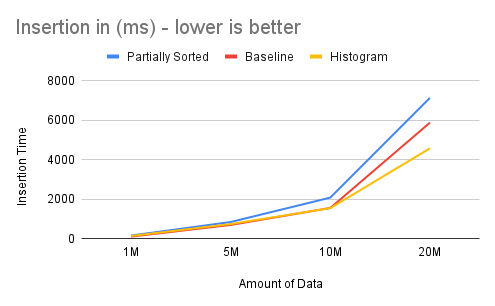
\includegraphics[width=100mm,scale=1]{Figures/InsertionResult.png}
    \caption{
Overall Insertion Operation vs Number of Insertion Operation Following Gaussian     Distribution.
    }
    \label{fig:GraphInsertionResult}
\end{figure}

The empirical analysis we conducted, which is presented in Table \ref{tab:InsertionResult} and Figure \ref{fig:GraphInsertionResult}, revealed that gap optimization using the histogram is a superior algorithm to the baseline with \acrshort{fmcd} \cite{LIPP} and partially sorted gapped array algorithms when the data follows Gaussian Distribution. This was evident from the performance gains realized by the histogram-based algorithm, which was able to capture the distribution of the data and distribute gaps based on the data's distribution, thus performing better than the \acrshort{lipp} when newly inserted data followed the same distribution as the existing data.

Moreover, the histogram-based algorithm's performance superiority over the baseline algorithm was found to widen as the amount of data stored in the \learnindex tree increased, as depicted in Figure \ref{fig:GraphInsertionResult}. This can be attributed to the histogram's efficient distribution of gaps in the data based on its distribution, which enables it to maintain optimal performance even with larger data sets.

Conversely, the partially sorted gapped array algorithm performed the worst among the three algorithms. This was mainly due to its requirement to perform a sequential search within the gapped array to locate empty spaces before inserting new data. As a result, the partially sorted algorithm's performance deteriorated as the amount of data stored in the \learnindex tree increased, as illustrated in Figure \ref{fig:GraphInsertionResult}. With larger amounts of data, there were more conflicts, which caused the partially sorted \learnindex to conduct more sequential searches, resulting in inferior performance compared to the baseline and histogram gap optimization algorithms.


\subsubsection{Lognormal Distribution}
\begin{table}
    \centering
    \begin{tabular}{ |p{2cm}|p{3cm}|p{3cm}|p{3cm}| } 
        
     \hline
     \multicolumn{4}{|c|}{Insertion Performance Result for Lognormal Distribution (in ms)} \\
     \hline
      Num Keys & Baseline (\acrshort{lipp})  & Partially Sorted & Histogram \\
     \hline
     \textbf{1M} & \cellcolor{green}127 & 156 & 199 \\
     \textbf{5M} & 1310 & 1593 & \cellcolor{green}1244 \\
     \textbf{10M} & 2593 & 3580 & \cellcolor{green}2443 \\
     \textbf{20M} & 5129 & 5930 & \cellcolor{green}4835 \\
     \hline
    
    \end{tabular}
     \caption{Insertion Results with Lognormal Distribution}
    \label{tab:InsertionResultLognormal}
\end{table}
\begin{figure}[H]
    \centering
    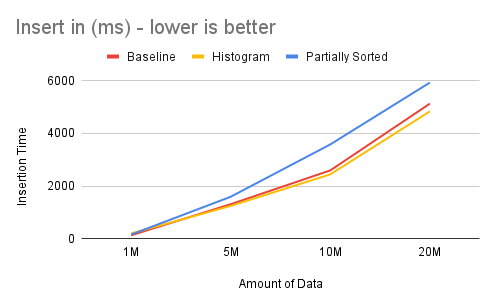
\includegraphics[width=100mm,scale=1]{Figures/InsertionResultLognormal.png}
    \caption{
     Overall Insertion Operation vs Number of Insertion Operation Following Lognormal Distribution.
    }
    \label{fig:GraphInsertionResultLognormal}
\end{figure}

Upon analyzing the results presented in Table \ref{tab:InsertionResultLognormal} and Figure \ref{fig:GraphInsertionResultLognormal}, we can conclude that the gap optimization using histogram algorithm still performs better than the baseline and partially sorted gapped array algorithms when using Log Normal Distribution. The results reveal that the histogram algorithm's superior performance is due to its ability to capture the distribution of the data and distribute gaps accordingly, thereby achieving better performance than the \acrshort{lipp} when the newly inserted data follows the same distribution as the existing data.

Similar to the findings with Gaussian Distribution, as the amount of data stored in the \learnindex tree increases, the performance gap between the histogram-based algorithm and the other two algorithms widens, as illustrated in Figure \ref{fig:GraphInsertionResultLognormal}. This can be attributed to the histogram algorithm's efficient distribution of gaps in the data, which enables it to maintain optimal performance even with larger data sets.

On the other hand, the partially sorted gapped array algorithm performed the worst among the three algorithms, as observed in the results presented in Figure \ref{fig:GraphInsertionResultLognormal}. The reason for this inferior performance can be attributed to the extra computations required to search for empty spaces after the predicted position. With larger amounts of data, the partially sorted algorithm's performance further deteriorates due to the increased amount of recursive rebuilding required when the spaces after the predicted position run out. Additionally, since each node contains more partially sorted items, each node takes longer to perform recursive rebuilding, leading to reduced performance as the amount of data increases.

The findings from our evaluation underscore the importance of considering the distribution of data when designing algorithms for processing and storing data. The results indicate that gap optimization using the histogram is a more efficient algorithm than the baseline and partially sorted gapped array algorithms, particularly when the newly inserted data follows the same distribution as the existing data. Leveraging techniques such as gap optimization using histograms can optimize performance and efficiency in data processing and storage.

\subsubsection{Powerlaw Distribution}

\begin{figure}[H]
    \centering
    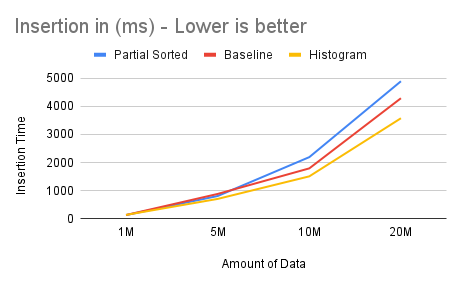
\includegraphics[width=100mm,scale=1]{Figures/InsertionResultPowerlaw.png}
    \caption{
    Overall Insertion Operation vs Number of Insertion Operation Following Powerlaw Distribution.
    }
    \label{fig:GraphInsertionResultPowerlaw}
\end{figure}
It is important to note that power-law distribution is different from the other distributions tested in that it has a long tail, meaning that there are a few elements that frequently occur while most elements are rare. This property can make it more challenging to capture the distribution using a histogram-based approach accurately.

Additionally, the wider spread of the performance gap in Figure \ref{fig:GraphInsertionResultPowerlaw} compared to the other distributions indicates that the insertion operation is more unpredictable in power-law distributed data. This may be due to the highly skewed nature of the distribution, making it difficult to predict where new elements should be inserted accurately.

Despite these challenges, the histogram-based gap optimization approach still outperforms the baseline and partially sorted gapped array in power-law distribution. This suggests that the approach is still effective in capturing the distribution and distributing gaps accordingly, leading to better insertion performance.

The poor performance of the partially sorted gapped array in power-law distribution further supports the idea that this approach is unsuitable for indexing this data type. As the amount of partially sorted keys in each node increases with larger datasets, the amount of recursive rebuilding required also increases, leading to worse performance.


\subsubsection{Real-World Dataset (Longitudes)}
\begin{figure}[H]
    \centering
    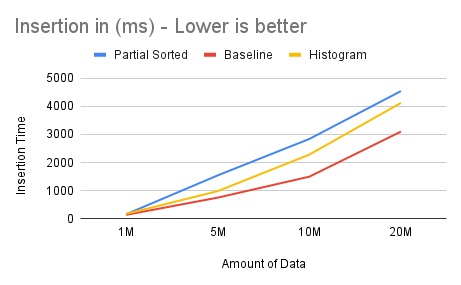
\includegraphics[width=100mm,scale=1]{Figures/InsertionResultLongitude.png}
    \caption{
       Overall Insertion Operation vs Number of Insertion Operation using Longitude Dataset.
    }
    \label{fig:GraphInsertionResultLongitude}
\end{figure}
To further analyze the result on a real-world dataset in Figure \ref{fig:GraphInsertionResultLongitude}, it is important to consider the nature of real-world data and how it can affect the performance of the algorithms. Real-world data is often diverse and can have a wide range of distributions, from uniform to skewed, and can also have varying degrees of correlation and clustering.

The baseline algorithm is able to perform better as it uses a \acrshort{fmcd} that distributes gaps and keys to optimize the linear regression model, and it does not require rebuilding during the insertion operation or does not have any assumption on the dataset. In other words, the baseline can be a good general purpose which performs well in any scenario. 

However, the histogram algorithm may not perform as well on real-world datasets as it does not account for the changing distribution of the data. The algorithm assumes that the data distribution is consistent and places gaps based on that assumption. This can lead to slower insertion times when the new data's distribution differs from the existing data.

Moreover, the partially sorted gapped array is not suitable for real-world datasets as it does not help the linear regression model improve its accuracy. Instead, it only delays the new node creation at a later stage to amortize the cost, which can be costly in terms of performance when there is a huge amount of data in the node.

The histogram algorithm is designed to work well when the distribution of the data is known, and it is able to adapt the gaps based on that distribution. But in real-world scenarios, where the distribution is not known or random, the baseline performs better as it is able to generalize to fit the randomness of the data. 

\subsection{Query}
To evaluate the performance of the query operation, we will test varying input sizes ranging from one million to twenty million, in order to determine which algorithms perform best in different scenarios and input sizes. Our tests will include both static (Gaussian, Lognormal, and Powerlaw) and dynamic (Longitudes) scenarios.

Testing static scenarios is important for query performance because it allows us to analyze the algorithms' behavior under specific data distributions. By using static datasets such as Gaussian, Lognormal and Powerlaw, we can evaluate how well the algorithms perform when the data follows a known distribution, and use this information to optimize the algorithm. For example, if an algorithm performs well on a Gaussian dataset, which is a commonly occurring distribution in real-world data, we can be confident that it will perform well on similar datasets in the future. This allows us to make more informed decisions when selecting which algorithms to use for specific tasks, and can help improve overall system performance.

Furthermore, testing static datasets allows us to measure the impact of the distribution on query performance, and identify any potential areas for optimization. This is particularly useful for algorithms that are designed to work with specific types of data distributions, such as the histogram-based algorithm that we tested earlier.

For each scenario, we will measure the query time taken by the baseline, histogram, and partially sorted algorithms. The results will be recorded and analyzed to determine which algorithm performs the best in each scenario.

This approach is necessary because different datasets may have different characteristics that affect the performance of the query operation. By testing different scenarios with varying input sizes, we can gain a better understanding of the strengths and weaknesses of each algorithm and determine which algorithm is the most suitable for a particular scenario.

Furthermore, by including both static and dynamic scenarios, we can compare the performance of the algorithms in scenarios where the data distribution is known beforehand and scenarios where the data distribution is constantly changing. This will provide valuable insights into the suitability of each algorithm in real-world scenarios where the data distribution is not known beforehand.

\subsubsection{Gaussian Distribution}
\begin{figure}[H]
    \centering
    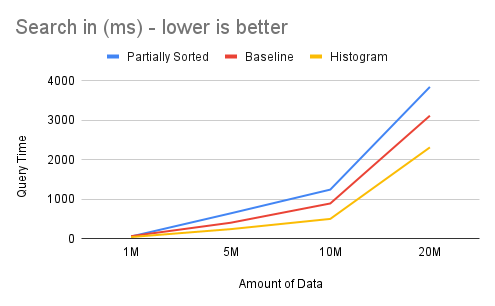
\includegraphics[width=100mm,scale=1]{Figures/QueryGaussian.png}
    \caption{
     Overall Query Operation vs Number of Query Operaton Following Gaussian Distribution
    }
    \label{fig:QueryResultGaussian}
\end{figure}
The results of the experiment show that the performance of \learnindex algorithms varies significantly depending on the distribution of the input data (Figure \ref{fig:QueryResultGaussian}). When it comes to query operations on the Gaussian Distribution, the histogram algorithm outperforms the other algorithms. This is because the histogram algorithm makes use of the gaps between keys that are specifically optimized for the given distribution. By doing so, it traverses lesser depth, which in turn improves the overall query performance.

On the other hand, the baseline algorithm performs relatively well compared to the partially sorted \learnindex algorithm. However, the baseline algorithm tries to generalize and perform well in most cases without taking advantage of the prior data distribution. This means its performance is less than the histogram algorithm in certain distribution types.

The partially sorted algorithm performs the worst of the other two algorithms in query operations. This is due to the extra computational overhead required when the keys are partially sorted. Even though the amount of conflicts is reduced with the partially sorted gapped array, the algorithm still spends a significant amount of time doing sequential searches due to potential miss predictions by the model and the partially sorted gapped array.

It is important to note that the above results were obtained in static scenarios, where the input data distribution remains constant. The histogram algorithm performed best in static scenarios because it was specifically optimized for the given distribution. 

\subsubsection{Lognormal Distribution}
\begin{figure}[H]
    \centering
    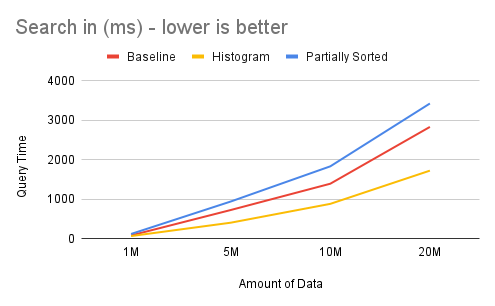
\includegraphics[width=100mm,scale=1]{Figures/QueryLognormal.png}
    \caption{
     Overall Query Operation vs Number of Query Operation Following Lognormal Distribution.
    }
    \label{fig:QueryResultLognormal}
\end{figure}
The experiment was also conducted on a lognormal distribution dataset. Similar to the Gaussian distribution (Figure \ref{fig:QueryResultLognormal}), the histogram algorithm outperformed the baseline \acrshort{lipp} and the partially sorted array in terms of query performance. The results shown in Figure 2 demonstrate that as the amount of data increases, the performance gap between the histogram and the baseline widens. This indicates that the histogram algorithm takes advantage of the data distribution and optimizes gaps in a way that allows the query to traverse fewer levels in the tree, leading to better performance.

On the other hand, the baseline algorithm still outperformed the partially sorted array even though the latter had a lower average tree depth. This is due to the extra computational overhead required for the $\epsilon$ linear search when there are a large number of partially sorted items in the tree. Despite having a lower average tree depth, the partially sorted array's slower search process prevented it from performing as well as the baseline in terms of query performance.

\subsubsection{Powerlaw Distribution}
\begin{figure}[H]
    \centering
    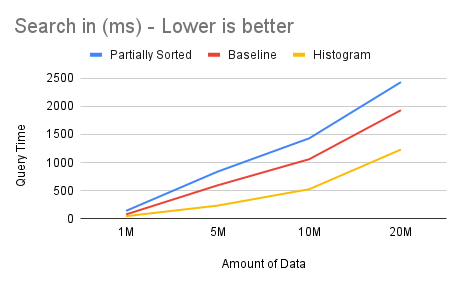
\includegraphics[width=100mm,scale=1]{Figures/QueryPowerlaw.png}
    \caption{
Overall Query Operation vs Number of Query Operation Following Powerlaw Distribution.
    }
    \label{fig:QueryResultPowerlaw}
\end{figure}
The study also evaluated the performance of the three data structures on Zipfian distribution (Figure \ref{fig:QueryResultPowerlaw}). The results were similar to the other distributions, with the histogram performing the best and the partially sorted gapped array performing the worst.

The histogram data structure again outperformed the baseline and partially sorted \learnindex structures due to its optimization for the Zipfian distribution. The gaps in the histogram structure are also specifically designed to account for the high frequency of certain keys in the distribution, resulting in a lower average tree depth and improved query performance.

In contrast, the baseline \learnindex performed relatively well in querying Zipfian distribution, but still could not match the efficiency of the histogram. This is because the baseline tries to generalize and perform well in most cases, but does not take full advantage of the specific distribution characteristics.

The partially sorted gapped array again struggled with the Zipfian distribution, with the extra computational overhead of the $\epsilon$ linear search causing a significant performance gap from the other two structures. As with the other distributions, the partially sorted \learnindex performed better than the baseline \learnindex in terms of average tree depth. However, this improvement was outweighed by the increased search time from the linear search.

\subsubsection{Real-World Dataset (Longitudes)}
\begin{figure}[H]
    \centering
    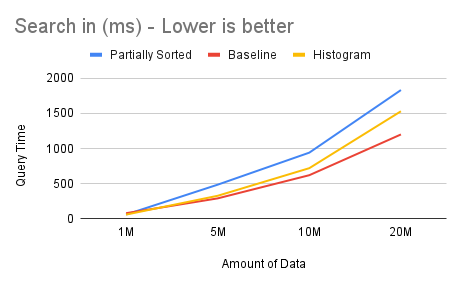
\includegraphics[width=100mm,scale=1]{Figures/QueryLongitude.png}
    \caption{
     Overall Query Operation vs Number of Query Operation using Longitude Dataset.
    }
    \label{fig:QueryResultLongitude}
\end{figure}
Moving to a real-world dataset, the experimental result in Figure \ref{fig:QueryResultLongitude} shows that the histogram performs on par with the baseline when it comes to range query. This indicates that both the baseline and histogram have a similar average tree depth which contributes to the similar query performance.

It is important to note that the query performance is heavily dependent on the height of the tree. If the tree height is greater, it leads to poor query performance. This can be attributed to the fact that a larger height would require the query algorithm to traverse through more levels of the tree, hence making the query more time-consuming.

However, when it comes to the partially sorted gapped array, the performance is still not up to the mark. Despite having a lower average tree depth compared to both baseline and histogram, the extra computation required for the linear search, after traversing the tree depth, hampers its overall query performance.


\subsection{Deletion}
In order to gain a deeper understanding of the performance of partially sorted and histograms compared to the baseline, we conduct further experiments involving delete operations. This setup is similar to the previous tests, with varying input sizes ranging from one to twenty million, using different distributions and a real-world dataset.

In the deletion operation, the performance is expected to be similar to that of the query operation, as the tree must be traversed to locate the keys before they can be deleted. This provides us with additional insight into the efficiency of each algorithm and how they handle deletions.

These experiments will allow us to further analyze the performance of each algorithm in different scenarios, providing a more comprehensive understanding of their strengths and weaknesses.

\subsubsection{Gaussian Distribution}
\begin{figure}[H]
    \centering
    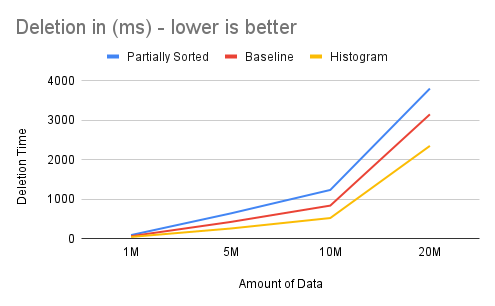
\includegraphics[width=100mm,scale=1]{Figures/DeleteGaussian.png}
    \caption{
Overall Deletion Operation vs Number of Deletion Operation Following Gaussian     Distribution.    }
    \label{fig:DeleteGaussian}
\end{figure}
The results Figure \ref{fig:DeleteGaussian} showed that the histogram outperformed both the baseline and the partially sorted array in Gaussian distribution. This was due to the lesser average depth of the tree, which made traversing down the tree faster, allowing for faster deletions.

It was also observed that the baseline still performed better than the partially sorted, even though it had a higher average tree depth compared to the partially sorted array. This was due to the precise position of the keys from the model and not requiring an extra linear search like the partially sorted gapped array. Furthermore, the sharp spike is due to increasing data from 10 M to 20 M.


\subsubsection{Powerlaw Distribution}
\begin{figure}[H]
    \centering
    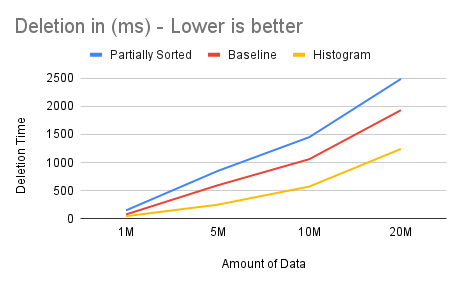
\includegraphics[width=100mm,scale=1]{Figures/DeletePowerlaw.png}
    \caption{
Overall Deletion Operation vs Number of Deletion Operation Following Powerlaw Distribution.
    }
    \label{fig:DeletePowerlaw}
\end{figure}
For the Powerlaw Distribution, we use a similar strategy as other distributions where we bulk load the keys and then insert the same amount into the tree. The resulting Figure \ref{fig:DeletePowerlaw} shows that the histogram still outperforms both baseline and partially sorted. The deletion works similarly to the query as it has to traverse down until it reaches a key before performing deletion which makes the deletion process bounded by the height of the tree. In this case, the reason why histogram achieve better performance is because it is able to make use of the gaps available in upper node and create lesser child node than the baseline. However partially sorted is slower even with similar tree depth is because it is bounded by the $\epsilon$ spaces and the height of the tree. The amount of time is mostly spent on the linear $\epsilon$ search which causes the gap in performance between the histogram and the partially sorted. 


Overall, the results in Figure \ref{fig:DeletePowerlaw} showed that the histogram indexing algorithm was consistently the best performer in terms of query, insertion, and deletion operations across various distributions and real-world datasets. However, it is worth noting that the baseline algorithm also performed relatively well and could be considered as a viable alternative in scenarios where the data distribution is unknown. On the other hand, the partially sorted gapped array algorithm performed poorly and could be improved by reducing the number of partially sorted keys in the gapped array.


\subsubsection{Real-World Dataset (Longitudes)}
\begin{figure}[H]
    \centering
    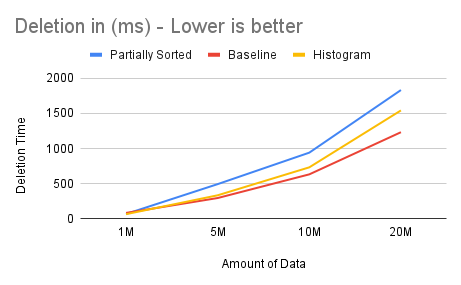
\includegraphics[width=100mm,scale=1]{Figures/DeleteLongitude.png}
    \caption{
    Overall Deletion Operation vs Number of Deletion Operation using Longitude Dataset.
    }
    \label{fig:DeleteLongitude}
\end{figure}
The real-world dataset serves as a more practical and relevant evaluation for these algorithms. The deletion operation is expected to have a similar performance to the query operation since both require traversing down the tree to locate the keys to be deleted or queriesd. As expected, the results in Figure \ref{fig:DeleteLongitude} show that the histogram and baseline perform similarly when deleting keys from the tree. This is due to their similar number of average tree height, which is a crucial factor that influences the query or deletion performance.

In contrast, the partially sorted gapped array performs worse than the histogram and baseline. Even though the partially sorted array has a lower average tree depth than the baseline, it requires an extra linear search after traversing down the tree to search for the predicted position of the key. This search is necessary because the keys could be located anywhere within a range of $x$ to $x + \epsilon$ around the predicted position. Consequently, the partially sorted array is bounded by the tree's height and the $\epsilon$ limit spaces after the predicted position. These factors contribute to its inferior performance compared to the histogram and baseline.


\subsection{Adjustment / Branch Pruning}
\begin{figure}[H]
    \centering
    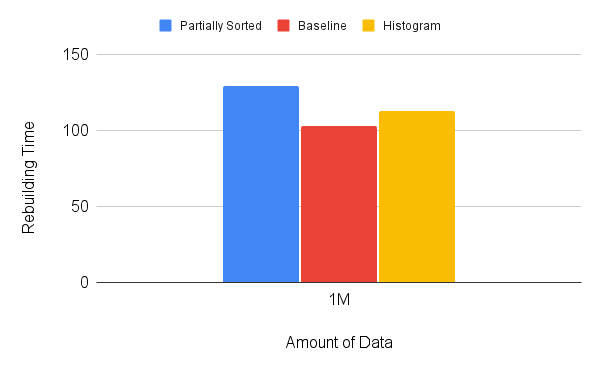
\includegraphics[width=100mm,scale=1]{Figures/RebuildingGaussian.png}
    \caption{
     Overall Rebuilding Time vs Amount of Keys in the Tree Following Gaussian Distribution
    }
    \label{fig:RebuildingGaussian}
\end{figure}
The \acrfull{lipp} algorithm is designed to optimize the performance of learned indexes by making adjustments to the tree's structure under specific conditions. These adjustments aim to reduce the tree's height, thereby reducing the time it takes to access and retrieve keys. During our testing of the learned indexes, we did not modify any of these conditions since they were already optimized for performance. However, we recognized that each of the algorithms (baseline, histogram, and partially sorted) has a unique implementation of these adjustments, which needed to be tested to determine the most effective implementation.

To test the effectiveness of these adjustments, we employed a rigorous testing strategy. We tested the algorithms on the Gaussian distribution dataset and measured the execution time in milliseconds. By comparing the performance of the three algorithms, we aimed to identify which implementation of the adjustments was most effective.

From the result Figure \ref{fig:RebuildingGaussian}, we observed that the histograms perform slower than the baseline on the test data. This is because the gap redistribution, retraining of the model, and rebuilding new histogram from the newly collected keys required for the histogram adjustments result in an operating cost of $O(N\log N)$. It costs the same as the baseline $O(N\log N)$ \cite{LIPP}, but the baseline does not need to rebuild the histogram, making it faster than the histogram algorithm. The partially sorted algorithm also performed worse than the baseline and histogram algorithms. This can be attributed to the challenges associated with collecting partially sorted keys. Nevertheless, like the histogram algorithm, the partially sorted algorithm's adjustments were also dominated by the retraining of the model and the collection of keys.



\section{Memory Consumption}
In addition to measuring the execution time, it is also essential to analyze the memory consumption of each implementation. Memory consumption refers to the amount of memory that is required to perform each operation. Therefore, in this section, we will be using the same data set as before but measuring the memory consumption of each implementation.

Measuring memory consumption is crucial as it helps us determine the amount of memory resources required to run each algorithm effectively. By analyzing the memory consumption, we can optimize the algorithm to reduce its memory footprint, which is important in scenarios where memory is a scarce resource.

We will use the same testing strategy as before, running each algorithm on the same data set and measuring the memory consumption in bytes. By comparing the memory consumption of the three algorithms, we can determine which implementation is the most memory-efficient.

It is important to note that memory consumption is affected by various factors, such as the size of the data set, the structure of  the data, and the algorithm's implementation. Therefore, the results obtained in this section will provide valuable insights into the memory consumption of each algorithm and help us optimize the algorithm for better performance.

\subsection{Gaussian Distribution}
\begin{figure}[H]
    \centering
    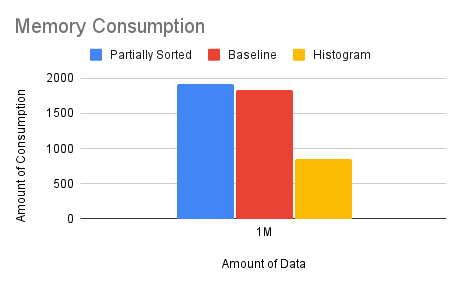
\includegraphics[width=100mm,scale=1]{Figures/MemoryGaussian.png}
    \caption{
     Results of Memory Consumption with Gaussian Dataset 1M
    }
    \label{fig:MemoryGaussian}
\end{figure}
From the result Figure \ref{fig:MemoryGaussian} of the test on Gaussian Distribution, we can observe that the histogram performs best in terms of memory consumption, consuming the least compared to the partially sorted array and the baseline. The reason behind this is that the histogram maintains an array of frequencies in each node, allowing it to capture the distribution of the keys. As a result, it can predict the exact position of a key without having to perform a linear search when there is a miss prediction, leading to fewer conflicts and the creation of fewer child nodes, ultimately reducing memory consumption. Even though, maintain frequencies in each node consumes extra memory but having lesser child node and average tree depth (Figure \ref{fig:AverageTreeDepthGau}) makes the histogram performs better in term of memory consumption.

In contrast, the partially sorted array performs worse than the histogram, even though the main idea behind the partially sorted is to delay the creation of child nodes as much as possible. As the data set grows, more partially sorted keys will be in each node. When a conflict occurs, and $\epsilon$ empty spaces run out, the algorithm still has to perform recursive rebuilding, creating numerous child nodes that consume memory. Therefore, the result is expected. 

Moreover, the baseline implementation performs similarly to the partially sorted. The baseline algorithm aims to work well in most scenarios, which makes it perform worse when there are assumptions that can be taken advantage of. From the result Figure \ref{fig:AverageTreeDepthGau}, we can see that the baseline creates more child nodes, which in turn consumes more memory than the partially sorted and histogram as the new nodes have to reserve some memory as \textsf{gaps} to be used for new keys.


\subsection{Powerlaw Distribution}
\begin{figure}[H]
    \centering
    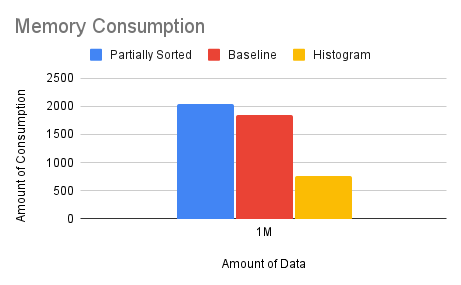
\includegraphics[width=100mm,scale=1]{Figures/MemoryPowerlaw.png}
    \caption{
     Results of Memory Consumption with Powerlaw Distribution Dataset 1M
    }
    \label{fig:MemoryPowerlaw}
\end{figure}
Our memory consumption test on the Powerlaw Distribution shows a similar trend to that of the Gaussian Distribution (Figure \ref{fig:MemoryPowerlaw}). The histogram outperforms both the baseline and partially sorted array in memory consumption. The histogram consumes less memory, making it more efficient for use in a static scenario where the data distribution is known. It is able to create fewer child nodes, utilizing the \textsf{gaps} efficiently.

On the other hand, the partially sorted array delays the creation of new nodes to amortize the cost. However, as the amount of data increases, it will eventually have to spend a significant amount of time rebuilding nodes recursively. This means that the number of nodes that need to be rebuilt will continue to increase as more data is added to the \learnindex.

Similarly, the baseline performs similarly to the partially sorted array. It does not make any assumptions about the data distribution, unlike the histogram, which creates more child nodes than the baseline.

\subsection{Lognormal Distribution}
\begin{figure}[H]
    \centering
    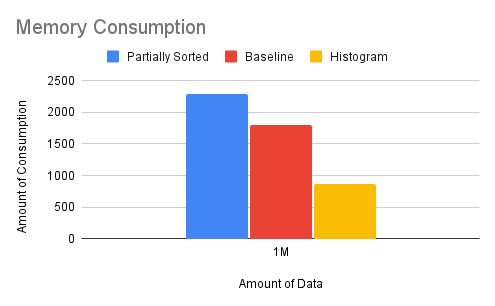
\includegraphics[width=100mm,scale=1]{Figures/MemoryLognormal.png}
    \caption{
     Results of Memory Consumption with Lognormal Distribution Dataset 1M
    }
    \label{fig:MemoryLognormal}
\end{figure}
The memory consumption test showed that the histogram outperformed the baseline and partially sorted \learnindex, which is consistent with the results from the Powerlaw Distribution (Figure \ref{fig:MemoryLognormal}). The histogram is able to maintain the distribution and gaps based on the data distribution, which allows it to have a lower average tree depth and consume less memory compared to the other two implementations.

On the other hand, the baseline only optimizes the keys based on the linear regression slope, which does not take into account the distribution of the data. As a result, it creates more child nodes and consumes more memory than the histogram. The partially sorted array delays the creation of new nodes to amortize the cost, but as the data becomes larger, it still needs to rebuild nodes recursively, resulting in more memory consumption.

Overall, the histogram is a more efficient implementation for static scenarios where the data distribution is known. Its ability to maintain gaps and distribution reduces the need for creating new child nodes and, thus, results in lower memory consumption.

\subsection{Real-World Dataset (Longitudes)}
\begin{figure}[H]
    \centering
    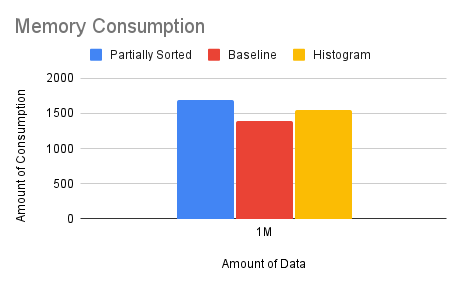
\includegraphics[width=100mm,scale=1]{Figures/MemoryLongitude.png}
    \caption{
     Results of Memory Consumption with Longitudes Distribution Dataset 1M
    }
    \label{fig:MemoryLongitude}
\end{figure}
However, for real-world scenarios where distribution is not known, the histogram performs worse than the baseline and is not able to capture the distribution of the data since the assumption is not valid for real-world data where distribution is known for newly insert keys (Figure \ref{fig:MemoryLongitude}). Since the histogram is not able to optimize based on the distribution, the histogram will cause more \conflict than the baseline which is expected and hence consume more memory. 

Similar to the histogram, the partially sorted method does not depend on any particular distribution. However, it defers resolving conflicts until all available empty spaces are filled, at which point it creates new child nodes. The results indicate that the partially sorted method performs slightly better than the histogram technique because it delays creating new nodes until a later stage. However, when there is a larger amount of data in the tree, the partially sorted method does consume more resources than the histogram. This is because it waits until the current node is completely filled before recursively rebuilding it, which uses up more memory.

When dealing with real-world datasets, it is better to use the baseline approach if memory consumption is a top priority. This method is highly adaptable and generally produces better outcomes than the histogram and partially sorted techniques. Nevertheless, if the data distribution is familiar, the histogram approach can be fine-tuned to better fit the data. 

\section{Number of New Node Creation / Tree depth}
In this section, we investigate the performance of three different \learnindex implementations, namely the histogram, partially sorted, and baseline, in terms of the number of new node creations or \conflict when using different datasets.

The number of \conflict is crucial in evaluating the performance of \learnindex algorithms, especially in dynamic scenarios, where the data distribution can change over time. For instance, when a new key is inserted into the tree, it may cause \conflict and result in new node creations to maintain the performance of the algorithm. Therefore, measuring the number of \conflict can provide insights into how well each \learnindex implementation adapts to changes in the data distribution.


We tested the three algorithms by performing bulk loading of one million to twenty million. After performing bulk loading we perform insertion for another one million to twenty million to test the trend and new node creation on different algorithms. Basically, we bulk load fifty percent of the keys in and insert another fifty percent later to perform the experiment, which means that one million will have two million in the tree. 


\subsection{Gaussian Distribution}
\begin{figure}[H]
    \centering
    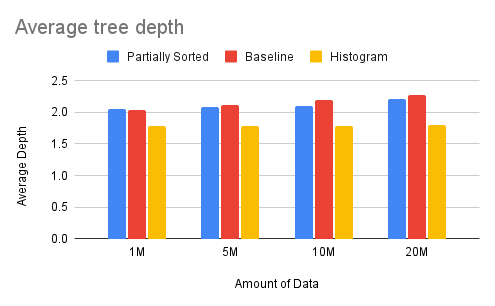
\includegraphics[width=100mm,scale=1]{Figures/AVGTD-Gau.png}
    \caption{
     Results of Average tree depth after a number of insertions (Gaussian)
    }
    \label{fig:AverageTreeDepthGau}
\end{figure}

From the results Figure \ref{fig:AverageTreeDepthGau}, we found that the histogram performs better on the average tree depth compared to the other two algorithms. Furthermore it has lesser \conflict number (new node creation) compared to partially sorted and baseline. This is because histogram is able to capture distributions of the data while partially sorted only delays \conflict until running out of space. This is inline with other experiments from previous sections. As lesser average tree depth improve operations performance as all of the operations are bounded by the height of the tree. For example, if we are able to reduce the depth of the tree, we will be able to reduce the time to perform read and write operations.

On the other hand, from result Figure \ref{fig:AverageTreeDepthGau}, the partially performs similarly to the baseline due, this is because the main idea of partially sorted is to store keys after the predicted position and reduce the number of new node creation. However, this is only delaying creating new node until later which will still be incured. This results inline with the operation experiments above as the amount of tree depth increase, the longer time it takes to perform read and write operation. Furthermore, the poor result on operations for partially sorted is due to the cost of recusively rebuilding the keys to be sorted.


In addition, the baseline performs worse than the histogram as the baseline implementation does not consider the data distribution, resulting in a higher number of average tree depth as it fails to optimize key positioning. From the results Figure \ref{fig:AverageTreeDepthGau}, can see that the baseline has higher average tree depth compared to histogram, which is inline with operations performance as histogram outperform the baseline in operations as well due to having lesser depth to traverse.



\subsection{Powerlaw Distribution}
\begin{figure}[H]
    \centering
    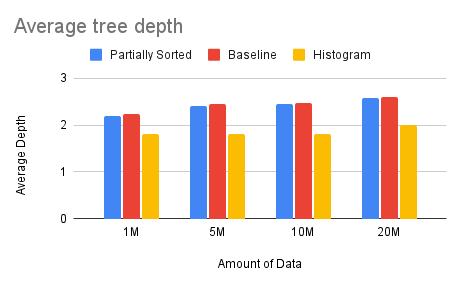
\includegraphics[width=100mm,scale=1]{Figures/AVGTD-Pow.png}
    \caption{
     Results of Average tree depth after a number of insertions (Powerlaw)
    }
    \label{fig:AverageTreeDepthPow}
\end{figure}
The result tested on Powerlaw distribution is not different from the Gaussian distribution (Figure \ref{fig:AverageTreeDepthPow}) where the histogram is able to outperforms both algorithm. This is because histogram can capture the distribution of the data and make use of the upper nodes gaps while the baseline just create new nodes whenever there is a \conflict and only wait until the next branch pruning (or adjustment) to occupy the upper nodes. 


Furthermore, partially sorted performs on par with the baseline as it only delays the new node creation until $\epsilon$ spaces runs out. From the result Figure \ref{fig:AverageTreeDepthPow}, we can see that the trend of average tree depth slowly increasing as more keys inserted in the tree. Even though the amount of data increase almost $10\times$, but the average tree depth does not increase much because of the branch pruning method that helps to reduce the amount of tree depth. However, we can see that the amount of average tree depth still increase for both partially sorted and baseline. While histogram is able to take advantage of the empty gaps in the upper node, which will create lesser new child node.

\subsection{Lognormal Distribution}
The result on Lognormal Distribution follows the same trend as previous distributions (Figure \ref{fig:AverageTreeDepthLog}). However the main difference from the previous test is that the baseline seem to have lesser average tree depth from five million to ten million, this is because when it reaches a condition, the baseline will trigger branch pruning which reduces the tree depth. 
\begin{figure}[H]
    \centering
    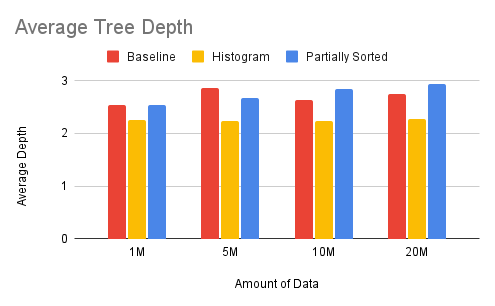
\includegraphics[width=100mm,scale=1]{Figures/AVGTD-Log.png}
    \caption{
     Results of Average tree depth after a number of insertions (Lognormal)
    }
    \label{fig:AverageTreeDepthLog}
\end{figure}

For histogram, we can see a similar trend where the histogram able to maintain the average tree height throughout the data increases. Which is inline with the result of insertion and search operations where it outperforms the baseline and partially sorted array. If it is able to make use of the upper nodes gaps, it will not need to wait until the branch pruning to make use of the available gaps in the upper nodes. 

\subsection{Real-World Dataset (Longitudes)}

On the other hand, the results on dynamic scenario (Figure \ref{fig:AverageTreeDepthLong}) shows that the baseline outperforms histogram and the partially sorted. Based from the result Figure \ref{fig:AverageTreeDepthLong}, we can see the baseline is able to make use of the gaps to insert and does not increase in the average depth while histogram does not perform when it comes to dynamic scenario as histogram can not capture the distribution which is crucial for histogram to work well. This results inline with the previous test on operations where baseline is able to out shine the histogram and partially sorted. This is because the search operation is only bounded by $O(h)$ where h is the height of the tree. This mean that reducing the amount of average tree depth will make the performance of the operations faster. 
Furthermore, the partially sorted perform similarly to both histogram and the baseline, as it make uses of the gaps by inserted keys after the predicted position which delays the new node creation, thus having lesser depth. 
\begin{figure}[H]
    \centering
    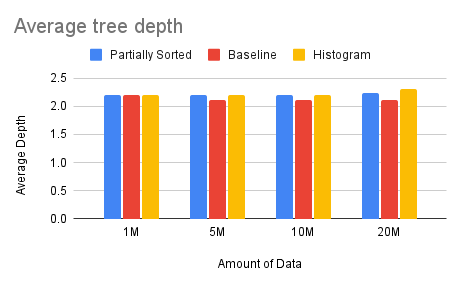
\includegraphics[width=100mm,scale=1]{Figures/AVGTD-Long.png}
    \caption{
     Results of Average tree depth after a number of insertions (Longitudes)
    }
    \label{fig:AverageTreeDepthLong}
\end{figure}
However this does not inline with the operations performance, this is because the operation performance of the partially sorted is bounded not just by the height of the tree, but also $\epsilon$ spaces. Which is similar to the section on \nameref{partialsortedtheory} where we mentioned that the time complexity of the operations is $O(\epsilon + \log N)$



\section{Evaluation Summary}
In this section, we have compared the performance of three learned index algorithms: baseline, histogram, and partially sorted. Our testing showed that the histogram implementation outperforms the baseline in operations such as insertion, deletion, and query when the distribution is static, and new keys follow the same distribution. This is due to the histogram's ability to minimize the height of the tree by grouping keys with similar values into a single bin, leading to faster traversal times.

In addition, measuring the number of \conflict can provide valuable insights into the performance of \learnindex algorithms in dynamic scenarios. The histogram implementation performs the best in terms of the number of \conflict, followed by the partially sorted implementation, while the baseline implementation performs the worst on the static scenario. On the other hand, the baseline outperforms the histogram and the partially sorted on the dynamic scenario. If the data distribution is known, histogram seems to be a better fit to optimize the gaps while performing faster on operations. If the data distribution is not known, baseline seem to perform better as it generalize to fit in many scenarios. Furthermore, the partially sorted still need more experiments and improve as the searches is still bounded by the extra search spaces after the predicted position which makes it slower during read and write operations.

However, our testing also revealed that the histogram implementation needed further exploration to improve its performance in real-world scenarios where data is not static and can change over time. This is an area where the partially sorted algorithm falls short, as it requires extra computation that causes operations to slow down as the data increases in the tree.

In conclusion, the choice of the learned index algorithm depends on the characteristics of the dataset being indexed and the expected usage patterns. For static distributions, the histogram algorithm offers the best performance, while the partially sorted algorithm may be more suitable for dynamic data. Nonetheless, further research is needed to explore the potential of these algorithms in more diverse scenarios and to develop more advanced learned index structures that can handle more complex data distributions. % Evaluation

\lhead{\emph{Study on Parameter Tuning}}

\chapter{Study on Parameter Tuning}
In this section, we will perform in depth analysis on different parameters and the trade off between the two algorithm (Histogram and Partially Sorted). Different parameters will yield different result and base on the different dataset. The experiment method will be the same as the evaluation section where we will be using the same dataset. However, we will only limits to real-world dataset and one of the distribution due to the computation power in testing all of the distribution. We expect that the result will help gain more understanding on different parameters that the histogram and partially sorted introduced and its flaws and tradeoff.

\section{Histogram Bin} \label{Histogram Bin}
\begin{figure}[H]
    \centering
    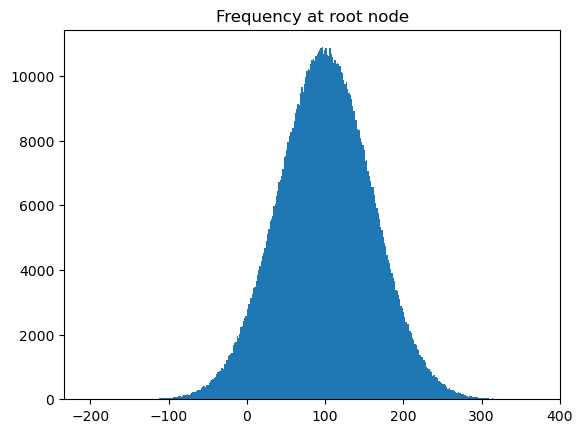
\includegraphics[width=100mm,scale=1]{Figures/GaussianDistributionRootNode.png}
    \caption{
     Distribution at root node
    }
    \label{fig:DistRootNode}
\end{figure}
The choice of the bin size is important consideration when maintaining a histogram in each node. The bin size determines the number of bins used in the histogram and the range of values includes in each bin. The bin size should be chosen carefully to ensure that the resulting histogram accurately reflects the distribution of the data. 

If the bin size is too small, the histogram may not be able to capture the distribution of keys in the node and difficult to interpret. This is because each bin will contain only a small number of data points, and the resulting bar heights will be highly variable. Which makes it difficult to see the underlying pattern of the data.  

On the other hand, if the bin size is too large, the resulting of the histogram in each node may be too coarse and may not accurately capture the fine details of the distribution. This will result in important details to be missed out. 

We tested small static bin and the \acrshort{fdrule} to gain some insights on the data patterns and how bins affect the gaps optimization. The figure \ref{fig:DistRootNode} is taken from the histogram \acrshort{lipp} root node with a Gaussian distribution dataset on one million keys. we can see that the root node will contain the whole tree distribution. 

In this section, we will test the static bin size and Freedman-Diaconis rule to find the appropriate bin size and its tradeoff using the same dataset and setup as the previous section. However, in our calculation of the $bin\_index$, we have to find the $bin\_width$ which determines the range of keys that fall into this index. For example, if $bin\_width$ is equal to $1$,  that means the range of first index can be in the range of keys $0$ to $1$. With static bin size, we can calculate $bin\_width$ by $\frac{Key_{max} - Key_{min}}{bin\_size}$.

\subsection{Gaussian Distribution} 
\begin{figure}[H]
    \centering
    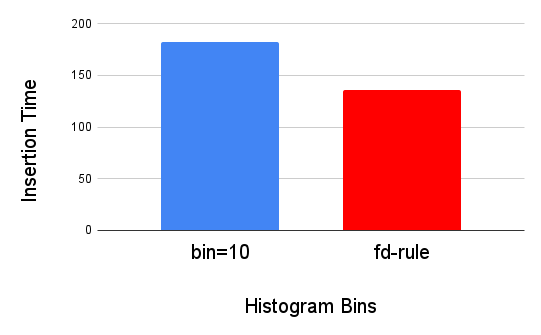
\includegraphics[width=100mm,scale=1]{Figures/InsertionHistBin.png}
    \caption{
     Results of Insertion on Different Histogram Bin Setting
    }
    \label{fig:InsertionHistBin}
\end{figure}
\begin{figure}[H]
    \centering
    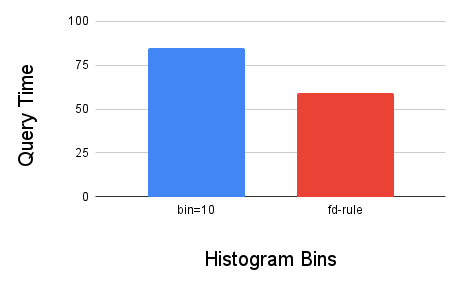
\includegraphics[width=100mm,scale=1]{Figures/QueryHistBin.png}
    \caption{
     Results of Query on Different Histogram Bin Setting
    }
    \label{fig:QueryHistBin}
\end{figure}
In this section, we aim to compare the performance of a static bin size of $10$ with the \acrshort{fdrule} when used in the histogram-based \learnindex algorithm on Gaussian Distribution. We carried out the same tests as in the previous section, but with the addition of comparing the performance of the different bin sizes.

From the resulting figure \ref{fig:InsertionHistBin} and \ref{fig:QueryHistBin}, we can observe that using a static bin size of $10$ does not perform well when there is a large amount of data in the tree. This is because the root node, which represents the entire distribution of the tree, does not capture the pattern well when the bin size is too small. As a result, the gap optimization in the tree performs poorly, causing the tree to grow deeper and impacting the read and write operations since they are bounded by $O(h)$ where $h$ is the height of the tree. Furthermore, we can also see that both the insertion and query operations perform poorly due to the increasing height of the tree when the gap optimization does not work well. Additionally, the number of \conflict (or new nodes created) also increases, as the histogram-based \learnindex relies heavily on the histogram in each node to distribute gaps according to the frequencies.
\begin{figure}[H]
    \centering
    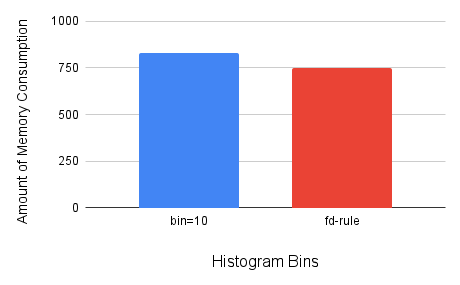
\includegraphics[width=100mm,scale=1]{Figures/MemoryHistBin.png}
    \caption{
     Results of Memory Consumption on different histogram bin setting
    }
    \label{fig:MemoryHistBin}
\end{figure}
In contrast, the \acrshort{fdrule} maintains a longer frequency (or bin) size, which consumes more memory compared to the static bin size. From the resulting figure \ref{fig:MemoryHistBin}, we can see that the \acrshort{fdrule} maintains larger number of bin sizes, while the static bin size only maintains $10$. This cost will be incurred when the adjustment triggers, and the algorithm has to rebuild the nodes. However, it offsets the operation cost, as the insertion operation has to traverse less depth compared to the static bin size. 

This makes the \acrshort{fdrule} performs well in term of representing the underlying patterns and able to make our gaps optimization works well on different distributions. It outperforms the static bin size when perform operations like the insertion, query and deletion due to the smaller depth that it has to traverse down.


\subsection{Real-World Dataset (Longitudes)} 
\begin{figure}[H]
    \centering
    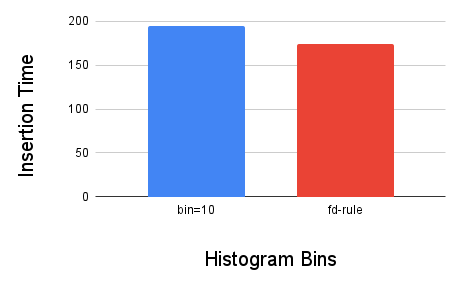
\includegraphics[width=100mm,scale=1]{Figures/InsertionHistBinLogi.png}
    \caption{
     Results of Insertion Operation on different histogram bin setting
    }
    \label{fig:InsertionResultLogi}
\end{figure}
Real-world datasets can have a complex distribution, and unlike synthetic datasets with known distributions, it can be challenging to predict the distribution of new keys. Therefore, it is important to evaluate the performance of the \learnindex algorithms on real-world datasets to understand how they adapt to the underlying patterns.

Based on the results of our experiments on real-world datasets, we observed that the performance of the histogram \learnindex was poor compared to the baseline, as discussed in the previous section. However, in this experiment, we evaluated the performance of two different approaches, namely the static bin size and the \acrshort{fdrule}.

The results showed that both the static bin size and the \acrshort{fdrule} did not perform well when the distribution of new keys was unknown, as they were not able to capture the underlying patterns of the dataset. As a result, both approaches performed poorly on insertion and query operations compared to the baseline. However, the \acrshort{fdrule} still outperforms the static bin size as it is able to capture keys' distribution better than the static bin size which overfits to only a few scenarios (Figure \ref{fig:InsertionResultLogi}).

\begin{figure}[H]
    \centering
    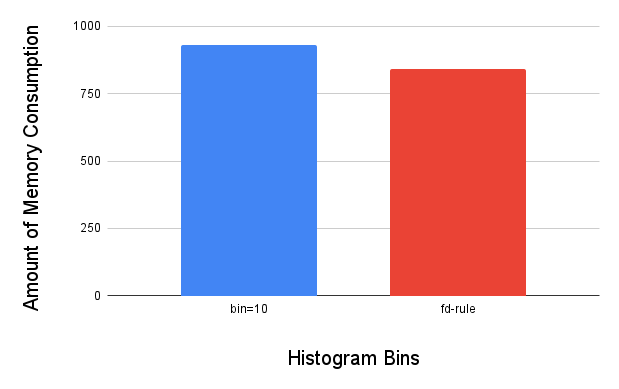
\includegraphics[width=100mm,scale=1]{Figures/MemoryHistBinLogi.png}
    \caption{
     Results of Memory Consumption on different histogram bin setting
    }
    \label{fig:MemoryConsumptionLogi}
\end{figure}

For memory consumption (Figure \ref{fig:MemoryConsumptionLogi}), the \acrshort{fdrule} still performs better than the static bin size. The \acrshort{fdrule} is able to capture the distribution better than the static bin size. Static bin size may only work in a few scenarios where there is not large amount of data. In this case, it makes static bin size create more child nodes than the \acrshort{fdrule} which consumes more memory to maintain the child nodes.

Therefore, based on our experiments on one million real-world keys, the \acrshort{fdrule} approach is a better solution for both real-world dataset and static dataset. This is because the \acrshort{fdrule} is able to capture distribution and distribute gaps based on the detailed distribution while the static bin size will only works if there is lesser data and require a lot of engineering efforts to tune this parameter to work on different scenarios. 



\section{Partially Sorted $\epsilon$ Spaces}
The $\epsilon$ spaces are a crucial factor in determining the performance of \learnindex, as it influences the traversal of the tree and the operation's runtime complexity. The $\epsilon$ parameter determines the number of gaps to search for in the gapped array when the predicted position is not empty. As all the operations are bounded by the $\epsilon$ spaces, the number of $\epsilon$ sets affects the search performance.

To determine the impact of the $\epsilon$ parameter on the search operation, we conducted experiments on different parameter values, namely $1$, $5$, and $10$, using the same datasets as in the previous section, i.e., Gaussian and Real-World datasets. We evaluated the performance of the insertion, query, and deletion operations using these different parameter values.

The $\epsilon$ parameter has a significant impact on the search operation's performance. In general, a larger value of $\epsilon$ will result in a higher number of gaps to search for, making the search operation more efficient as query has to traverse down lesser depth due to smaller tree heigit. However, a larger value of $\epsilon$ also increases the memory overhead of the index, as more gaps need to be stored. 

On the other hand, a smaller value of $\epsilon$ will result in fewer gaps to search for, making the new node creation higher which will make the search operation in efficient. However, a smaller value of $\epsilon$ also reduces the number of search after the non-empty spaces.


\subsection{Gaussian Distribution}
\begin{figure}[H]
    \centering
    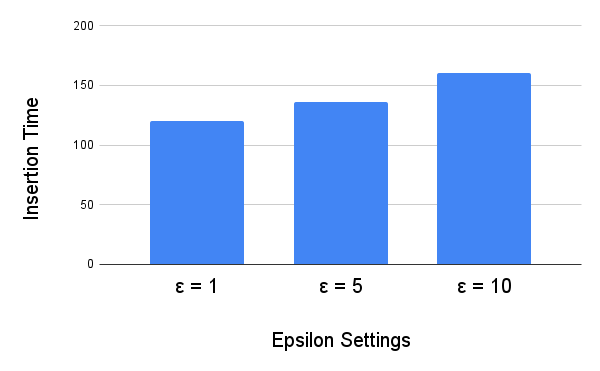
\includegraphics[width=100mm,scale=1]{Figures/InsertionGauEp.png}
    \caption{
     Results of Insertion Operation on different Partially Sorted $\epsilon$ spaces
    }
    \label{fig:InsertionGauEp}
\end{figure}
\begin{figure}[H]
    \centering
    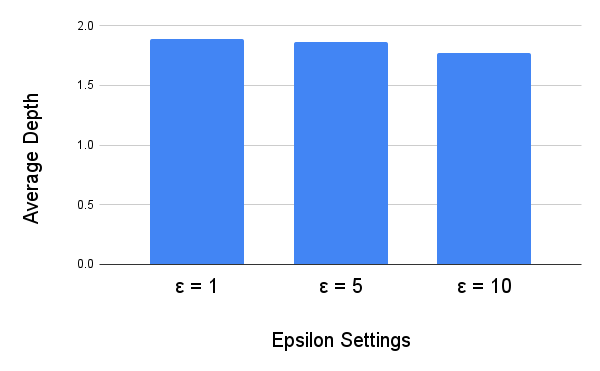
\includegraphics[width=100mm,scale=1]{Figures/AvgTreeEpGau.png}
    \caption{
     Results of Average Tree Depth on different Partially Sorted $\epsilon$ spaces
    }
    \label{fig:AverageTreeDepthGauEp}
\end{figure}
In the case of the Gaussian Distribution, we inserted keys with the same distribution as the keys that were already present in the tree. However, we do not expect the partially sorted data structure to perform well on this distribution as it only delays the slow operation of new node creation until the gaps are full. The results from the Insertion operation Figure \ref{fig:InsertionGauEp} shows that the trend of results changes as the number of $\epsilon$ decreases, indicating that the insertion operation becomes faster as the number of searches it has to perform decreases. However, if we look at the Figure \ref{fig:AverageTreeDepthGauEp}, we can see that the number of new node creations increases as the number of $\epsilon$ decreases. This is because it has lesser $\epsilon$ spaces for the partially sorted to delay new node creation. 

In addition, querying keys in the partially sorted data structure has the same performance trend as the insertion operation. This is because they both have the same time complexity, which is $O(\epsilon+\log N)$. This complexity is bounded by the search after the predicted position. Based on our results, it seems that the time to search a key is mostly dominated by the $\epsilon$ linear search as the trend of the search performance seem to decreases while the $\epsilon$ also decreases. However the number of nodes creation inversely related to the $\epsilon$ because the smaller the $\epsilon$, the number of lesser gaps to delay new node creation. 

The importance of the $\epsilon$ parameter in the partially sorted data structure is enormous, as all operations are mostly bounded by the traversals down the tree height and the $\epsilon$ spaces (or $O(\epsilon+\log N)$). The $\epsilon$ parameter determines the number of gaps in the gapped array to search for when the predicted position is not empty. Since all operations are bounded by the $\epsilon$ spaces, the number of $\epsilon$ sets will affect the search performance. 

Furthermore, its effectiveness heavily depends on the choice of the parameter $\epsilon$, which determines the number of gaps to search for when the predicted position of a key is not empty. This choice can require significant engineering effort, and even with a well-chosen $\epsilon$, partially sorted may not outperform other data structures.

In comparison to baseline and histogram data structures, which are only bounded by the height of the tree, partially sorted suffers from the need to delay the creation of new nodes until gaps are filled. This means that partially sorted does not assume any underlying pattern in the data distribution, but instead aims to optimize search and insertion by using the gaps as a buffer.

\subsection{Real-World Dataset (Longitudes)} 
\begin{figure}[H]
    \centering
    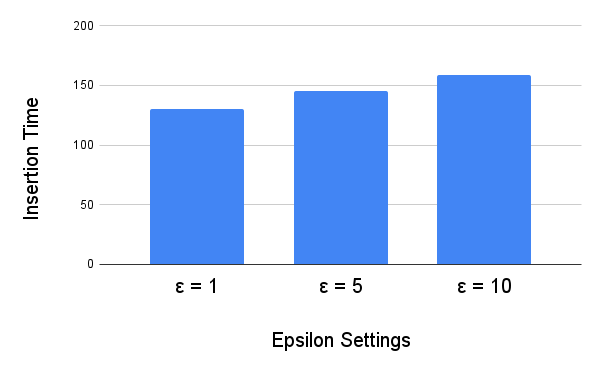
\includegraphics[width=100mm,scale=1]{Figures/InsertionLogEp.png}
    \caption{
     Results of Insertion Operation on Different Partially Sorted $\epsilon$ Spaces 
    }
    \label{fig:InsertionLogEp}
\end{figure}
\begin{figure}[H]
    \centering
    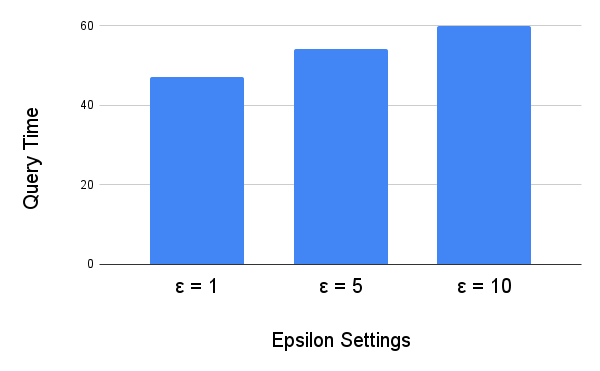
\includegraphics[width=100mm,scale=1]{Figures/QueryLogEp.png}
    \caption{
     Results of Query Operation on Different Partially Sorted $\epsilon$ Spaces 
    }
    \label{fig:QueryLogEp}
\end{figure}
When applied to real-world datasets, the partially sorted algorithm demonstrates a similar performance trend to that seen in static scenarios. When compared to other algorithms such as baseline and histogram, the partially sorted algorithm may not always be the most efficient. Nevertheless, this section of our study focuses on comparing the performance of different partially sorted parameter settings.

The results presented in the figure \ref{fig:InsertionLogEp} and \ref{fig:QueryLogEp} clearly show that partially sorted with $\epsilon = 1$ performs best in operations such as insertion, deletion, and query. This is because this setting only requires one space search after the predicted position, which can significantly improve the algorithm's performance. Since the time complexity of the algorithm is bounded by $\epsilon+\log N$, a lower value of $\epsilon$ leads to faster operations.
\begin{figure}[H]
    \centering
    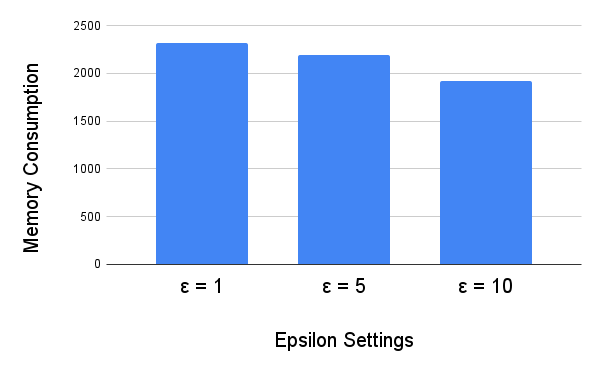
\includegraphics[width=100mm,scale=1]{Figures/MemoryLogEp.png}
    \caption{
     Results of Memory Consumption on Different Partially Sorted $\epsilon$ Spaces 
    }
    \label{fig:MemoryLogEp}
\end{figure}
However, when $\epsilon$ is decreased, the memory consumption of the algorithm increases (Figure \ref{fig:MemoryLogEp}). This is in line with our expectations, as reducing the number of spaces only delays the new node creation process for one conflict. As a result, there are more child nodes with lower $\epsilon$ values, leading to increased memory usage.

In summary, the value of $\epsilon$ in partially sorted refers to the number of limits that the algorithm can locate, which only delays the new node creation process. This algorithm does not take advantage of the underlying pattern of the keys, making its results similar for both real-world datasets and static scenarios. Therefore, selecting the optimal value of $\epsilon$ for a given dataset is critical to achieving the best performance of the partially sorted algorithm.

\section{Tradeoff}
Tradeoff is a crucial aspect of designing a \learnindex structure as it involves balancing size, accuracy, and efficiency. However, the accuracy can be eliminated by introducing new node creation in \acrshort{lipp} algorithm \cite{LIPP}, which leads to exact predictions but increases the size of the structure as a new node is created each time the predicted location is already occupied. In contrast, the partially sorted algorithm introduces the accuracy tradeoff in terms of $\epsilon$ which determines the number of keys that can be located in the structure.

In this section, we will compare the tradeoffs between Histogram and Partially Sorted parameters using the results obtained in the previous section. Although the Histogram algorithm does not require an accuracy tradeoff as the predicted position is exact and the time complexity is bounded by the height of the tree. In contrast, Partially Sorted provides a balance between accuracy, size and efficiency tradeoffs, but it may not perform as efficiently as Histogram or other algorithms in certain scenarios. Therefore, it is important to consider the specific use case and requirements when deciding which algorithm to use.

\subsection{Histogram}
In the previous section on \nameref{Histogram Bin}, we compared the performance of different bin sizes in a static scenario with a Gaussian Distribution. We found that the histogram outperformed the baseline and partially sorted algorithms. However, we also found that the choice of bin size plays a significant role in the accuracy and efficiency of the algorithm. If the bin size is too small, the histogram will not be able to capture the distribution of keys in the tree, resulting in poor accuracy. On the other hand, if the bin size is too large, the distribution will be too coarse, also resulting in poor accuracy. Hence, there is a tradeoff between bin size and the visibility of underlying patterns.

In terms of memory consumption, a \acrshort{fdrule} is the best option. However, this approach sacrifices the node size as it has to maintain higher size of frequencies array. Furthermore, the static bin size require fine tuning which consequently lead to more conflicts, and the \learnindex will have to create more new nodes, making operations less efficient. Tuning for a good enough bin size becomes challenging as the tree grows larger, and each node has its own distribution, which cannot use a "one size fits all" approach. However, if we compare with the baseline, the histogram algorithm consumes more memory as it has to maintain the frequency array to distribute gaps while baseline does not have extra array in each node.

In addition, \acrshort{fdrule} helps determine the bin size based on the keys in each node. This approach decides the bin size in each node such that it is good enough to distribute gaps based on the frequencies array. However, the tradeoff for this implementation is that it will consume more memory in each node as it has to maintain the array of frequencies. Due to variable bin size, the accuracy of distributing gaps increases, which decreases the number of conflicts. Thus, operations performance increases, as seen from the previous section.

From our experiment, we conclude that using \acrshort{fdrule} is the best approach as it determines a good enough bin size for each node, resulting in higher accuracy and fewer conflicts. However, controlling the amount of memory consumption can be challenging. It is essential to balance memory consumption and performance to achieve the optimal solution. We argue that optimizing operations performance is the best approach since insertion and query operations occur frequently in real-world systems where users have to keep the data updated. Thus, the efficiency of these operations plays a critical role in the overall system performance.


\subsection{Partially Sorted} 
In this section, we discuss the tradeoff between size, efficiency and accuracy in the context of \learnindex with partially sorted arrays. Unlike histogram bins, partially sorted arrays use the concept of partial limit spaces or $\epsilon$ to delay the slow new node creation by storing it a few $\epsilon$ spaces after predicted position. $\epsilon$ defines the number of spaces that the algorithm has to search for after the predicted position. Therefore, the operation performance like insertion is bounded by $\epsilon + \log N$, where $N$ is the number of keys in the node. In this section, we will be experimenting with different values of $\epsilon$ to determine the tradeoff between size, efficiency, and accuracy.

From the experimental results in Figure \ref{fig:InsertionGauEp}, we observe that the operation performance of partially sorted arrays decreases as $\epsilon$ increases. This is consistent with the theoretical analysis that suggests that the performance is not only bounded by $\log N$, but also by the $\epsilon$ spaces that the algorithm has to search. On the other hand, partially sorted arrays do not need to store any extra information like histogram bins, where a frequency array is maintained for each node. To determine if a key is partially sorted or not, we simply use the model to predict the position of the key and compare it with the current position. If the predicted position is different from the current position, then it is a partially sorted key.

In terms of operation performance, we observe that insertion is the most impacted operation by the choice of $\epsilon$. The reason for this is the recursive rebuild operation that is triggered when the $\epsilon$ spaces are exhausted. In particular, when the number of partially sorted keys in the node is high, the number of recursive rebuild operations required also increases, thereby reducing the efficiency of the insertion operation.

Based on the experimental results, we can conclude that $\epsilon = 1$ offers the best tradeoff between size and performance in terms of operations like insertion. However, as $\epsilon$ increases, the performance of the partially sorted array also improves, but at the cost of increased memory consumption due to the need to store more partially sorted keys. For example, when $\epsilon = 5$, the performance of insertion is significantly worse than when $\epsilon = 1$ due to the increased number of recursive rebuild operations required to insert a new key.

In conclusion, the choice of $\epsilon$ in partially sorted arrays determines the tradeoff between size, efficiency, and accuracy. While a smaller value of $\epsilon$ improves the performance of operations like insertion, a larger value of $\epsilon$ improves the memory consumption of the algorithm at the cost of increases in operation time. Therefore, it is important to strike a balance between these tradeoffs when implementing \learnindex with partially sorted arrays.



\section{Maximum Gaps}
In this section, we will delve deeper into an experiment to explore how different gaps distributions affect the performance and memory consumption of Histograms. This experiment is essential because the number of gaps that we distribute will affect the overall usage of memory as the gaps have to be reserved for key insertion.

In this experiment, we will test different datasets, such as Gaussian distributions and real-world datasets, to observe the changing trends and the trade-offs on different settings of gap distribution. We will also test different gap distributions such as $2\times$, $2.5\times$, and $3\times$. The $2\times$ refers to double the size of keys currently collected in the adjustments. The adjustment or branch pruning is only done based on the mentioned condition. For example, if we collected keys of $[1,2,3]$, the size of the expanded array will be $2\times 3$ which is $6$ so there will be $3$ keys and $3$ gaps. However, for $2.5\times$ the size, if the outcome of multiplication contains a decimal, we will round it up and place the leftover gaps at the end of the array.

\begin{figure}[H]
    \centering
    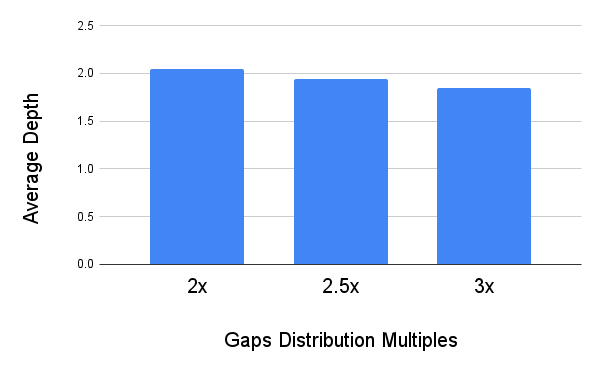
\includegraphics[width=100mm,scale=1]{Figures/AVGGauMaxGaps.png}
    \caption{
     Results of Average Tree Height on Different Maximum Gaps Parameters (Gaussian Distribution)
    }
    \label{fig:AvgMaxGapsGau}
\end{figure}
In the experiment on the Gaussian distribution, the results in figure \ref{fig:AvgMaxGapsGau} show that distributing gaps $3\times$ the size of keys collected performs best in terms of new node creation, as it has more gaps to locate keys in, which will reduce the number of child nodes. This setting can also increase the operation performance like insertion, as it traverses to a lesser depth than the $2\times$ and $2.5\times$ settings.
\begin{figure}[H]
    \centering
    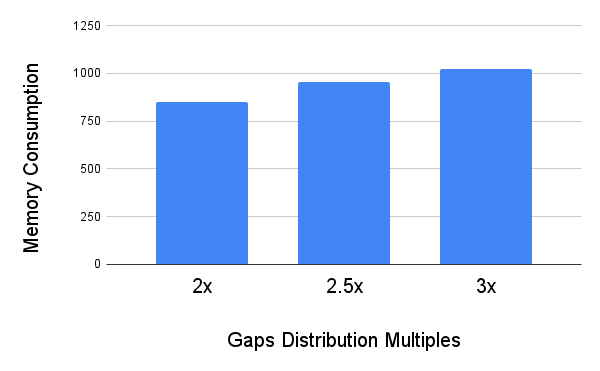
\includegraphics[width=100mm,scale=1]{Figures/MemoryMaxGapsGau.png}
    \caption{
     Results of Memory Consumption on Different Maximum Gaps Parameters (Gaussian Distribution)
    }
    \label{fig:MemoryMaxGapsGau}
\end{figure}
However, the memory consumption is affected by the increasing number of gaps, which is a tradeoff between size and efficiency. From the memory consumption figure \ref{fig:MemoryMaxGapsGau}, we can see that the amount of memory consumed by $3\times$ increases from $2\times$ and $2.5\times$. Even though $3\times$ has lesser tree depth, but reserving more gaps in each nodes consumes more memory than the amount of new child nodes created by $2\times$.

If the operation performance is the main concern, distributing more gaps can help reduce the number of new node creations while consuming more memory, as the gaps must be reserved for new keys, which is in line with the theoretical analysis that the performance is bounded by the height of the tree ($O(\log N)$). That means if we can reduce the height of the tree, we will gain performance in operations like insertion, deletion, and query. However, if memory is the primary concern, distributing more gaps will consume more memory.

From our testing, it seems that the $2\times$ setting is the best tradeoff between operation performance and memory consumption, as the average tree height trend does not increase as much as the memory consumption. From the figure \ref{fig:MemoryMaxGapsGau}, we can see that the $3\times$ gaps distribution increases memory consumption much more than it increases operation performance. Which makes $2\times$ the best tradeoff in performance and size. 
\begin{figure}[H]
    \centering
    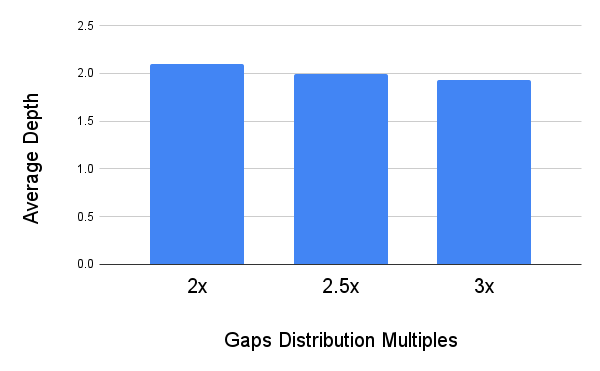
\includegraphics[width=100mm,scale=1]{Figures/AvgLogMaxGaps.png}
    \caption{
     Results of Average Tree Height on different Maximum Gaps Parameters (Longitudes Distribution)
    }
    \label{fig:AvgLogMaxGaps}
\end{figure}
For the real-world dataset, a similar trend appears that the maximum number of gaps to distribute will have more gaps for the model to insert new keys into. Based on the figure \ref{fig:AvgLogMaxGaps}, we can see that the $3\times$ performs better in terms of average tree height as it reduces the number of new child nodes because it has more gaps for the machine learn index to place new keys in. When there are fewer child nodes, the operation performance increases, which is in line with the theoretical analysis, where the operation performance for histograms is bounded by how much the height of the tree grows.
\begin{figure}[H]
    \centering
    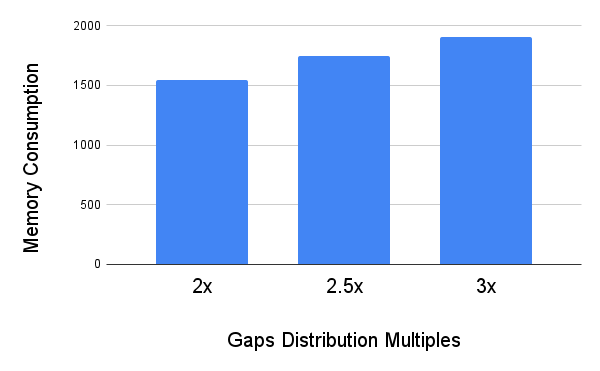
\includegraphics[width=100mm,scale=1]{Figures/MemoryLogMaxGaps.png}
    \caption{
     Results of Memory Consumption on different Maximum Gaps Parameters (Longitudes Distribution)
    }
    \label{fig:MemoryLogMaxGaps}
\end{figure}
However, expanding more gaps $3\times$ consumes extra memory (figure \ref{fig:MemoryLogMaxGaps}) as the gaps have to be reserved for new keys, which will consume memory. Furthermore, we can see from the figure \ref{fig:MemoryLogMaxGaps} that the amount of memory consumption increases when we distribute more gaps. However, the gain in operation performance is not significant and does not outweigh the fact that memory consumption trend increases higher than the operation performance. Which makes $2\times$ the number of collected keys the best tradeoff between operation performance and memory consumption in real-world datasets.

In conclusion, distributing more gaps can help reduce the number of new node creations and increase operation performance, but at the expense of memory consumption. The optimal gap distribution is a tradeoff between operation performance and memory consumption, with $2\times$ being the best setting for most scenarios.

\section{Scalability}

In this section, we will delve into the scalability of two indexing algorithms, namely the histogram and partially sorted index, by analyzing their performance on datasets of varying sizes. We will be using the same datasets as the previous section, but this time with an increase in the number of insertions. We will test on datasets with sizes of $10M$, $20M$, and $50M$ and also perform tests on both Gaussian distribution and real-world datasets.

The performance of an indexing algorithm is crucial when dealing with large datasets as it determines the speed of insertion, query, and building. A good indexing algorithm should be able to handle large datasets efficiently, without sacrificing performance. The scalability of an indexing algorithm is, therefore, an important factor to consider when selecting an indexing algorithm.

To test the scalability of the histogram and partially sorted index, we will perform insertion, query, and building operations on datasets of varying sizes. We will start by inserting $10M$ keys into both indexing algorithms and measure their performance. We will then repeat the process with datasets of sizes $20M$ and $50M$.

Additionally, we will test the scalability of the algorithms on two different types of datasets. The first type is the Gaussian distribution, which is a well-known distribution often used to test algorithms. The second type is a real-world dataset, which is more complex and closer to the kind of data an algorithm would encounter in a practical scenario.
\begin{figure}[H]
    \centering
    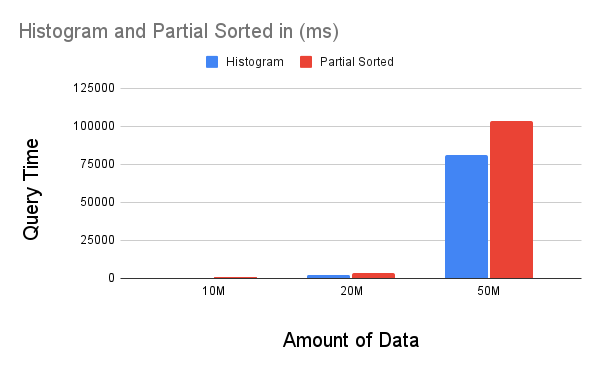
\includegraphics[width=100mm,scale=1]{Figures/QueryScalability.png}
    \caption{
     Results of Query Operation on different test sizes (Gaussian Distribution)
    }
    \label{fig:QueryScalability}
\end{figure}
When it comes to query performance on Gaussian Distribution, the histogram has a clear advantage over the partially sorted approach (Figure \ref{fig:QueryScalability}). This is because the histogram, as an extension of \acrshort{lipp}, only needs to traverse down the tree depth to locate the keys, while partially sorted requires a search just like other \learnindex algorithms. In our tests using the Gaussian Distribution dataset, we found that query time increases as the amount of data increases and the tree height grows larger for the histogram. This is consistent with the theoretical prediction that query time is bounded by the height of the tree.

On the other hand, the partially sorted approach showed the highest growth rate compared to the baseline and histogram. This is because the algorithm has to perform a local search for $\epsilon$ after traversing down the tree depth. As per the theoretical analysis, query time is bounded by $O(\epsilon + \log N)$, which makes the partially sorted approach not scalable as the amount of data increases. When there are many partially sorted keys within each node, the performance of the partially sorted approach is affected, which makes it slower than other \learnindex algorithms.
\begin{figure}[H]
    \centering
    \includegraphics[width=100mm,scale=1]{Figures/InsertionScalability.png}
    \caption{
     Results of Insertion Operation on different test sizes (Gaussian Distribution)
    }
    \label{fig:InsertionScalability}
\end{figure}
Insertion time shows a similar trend to query performance (Figure \ref{fig:InsertionScalability}), where the histogram outperforms the partially sorted approach as the data size increases. When the data size is small, the partially sorted approach tends to outperform the histogram because it delays new node creation, while the histogram creates a new node only when there is a conflict. However, when the amount of data increases, and more partially sorted keys are inserted into each node, the performance of the partially sorted approach worsens as it has to perform recursive rebuilding. This slows down the insertion performance compared to the histogram since the recursive rebuilding cost is $O(\frac{N}{2})$, where $N$ is the number of keys in the node.

When it comes to query and insertion performance in real-world datasets, we have seen that the histogram approach may not be as effective as it is in the Gaussian distribution. However, the general trend of histogram outperforming partially sorted is still observed. This is because, in histogram, we only need to traverse down the tree depth to locate the keys, whereas in partially sorted, we need to perform local search similar to \acrshort{alex}\cite{ALEX}. As the amount of data increases, the number of partially sorted keys also increases, which in turn increases the depth of the tree. Therefore, we observe a linear increase in partially sorted performance with increasing data size. However, histogram can still create new nodes and increase the tree depth without the need for local search, making it more scalable than the partially sorted approach.

Furthermore, the trend in insertion performance is also similar to that of query performance. When the amount of data is small, partially sorted tends to outperform the histogram as it delays the creation of new nodes. However, as more data is inserted into the tree, the number of partially sorted keys in each node increases, which triggers recursive rebuilding that can slow down the insertion performance. In contrast, the histogram approach still outperforms partially sorted because it only needs to traverse down the tree depth and create new nodes when there is a conflict, without the need for local search. This makes the insertion operation faster in histogram than in partially sorted.

In summary, the histogram approach is more scalable than the partially sorted approach for both query and insertion operations, especially when dealing with large amounts of data, as histogram does not require any extra searches after traversing down the tree compared to partially sorted keys.
 % Experimental Analysis

\lhead{\emph{Conclusion}}




\chapter{Conclusion}
\section{Contributions}
In summary, this thesis proposes two new strategies to optimize \learnindex: the Histogram and Partially Sorted Insertion Strategy. The Histogram method aims to capture the distribution and pattern of the data by maintaining a frequency array in each node. The gaps are distributed where they are needed the most, based on the data distribution, which helps to minimize the number of child nodes and improve the operation performance.

The Partially Sorted Insertion Strategy works by delaying the creation of new nodes until the amount of $\epsilon$ is full. This approach helps to reduce the number of child nodes created and optimize the memory consumption of the \learnindex.

To evaluate the performance of the proposed methods, we conducted experiments on various parameters such as memory consumption, the number of child nodes, and operation performance, and compared the results with the baseline \acrshort{lipp} method. The experiments show that the Histogram outperform the baseline \acrshort{lipp} method and partially sorted insertion strategy in terms of memory consumption and operation performance by up to \textbf{$2\times - 3\times$}. We hope that our algorithms complement the existing studies on the dynamic learned index.

\section{Limitations}
Despite the advantages of the histogram and partially sorted, there are still some limitations to consider. One limitation of the histogram is its performance on real-world datasets, where it does not capture the distribution as well as the raw \acrshort{lipp}. This is because histogram creates child nodes whenever there is a conflict, which can significantly affect the operation performance. In contrast, \acrshort{lipp} creates less child nodes and performs better in capturing the distribution of real-world datasets.

Another limitation of partially sorted is that it still does not perform as well as \acrshort{lipp} and histogram due to the extra local search that it has to perform. While partially sorted delays new node creation, it requires additional operations to maintain its partially sorted property, making it slower than \acrshort{lipp} and histogram. Additionally, our research mainly focuses on the efficiency and memory consumption of these \learnindex structures, without delving into their model accuracy. Future research could explore the triangular tradeoff between model accuracy, size, and efficiency in partially sorted.

In summary, while histogram and partially sorted have advantages over other \learnindex structures, they still have limitations that need to be considered. Understanding these limitations can help researchers and practitioners choose the best \learnindex structure for their specific use case.

\section{Future Work}
In this section, we put forward some potential avenues for future research that could enhance both the histogram and partially sorted array, with the goal of further improving the performance of the \learnindex. By doing so, we hope to provide guidance for future studies that can build upon our findings and push the limits of what is possible with the \learnindex.
\subsection{Histogram}
 One limitation of the histogram is that it assumes the dataset has a fixed and known distribution. In practice, this is often not the case, as real-world datasets may have outliers and do not follow a known distribution. This limitation can affect the accuracy of the histogram, leading to suboptimal query processing performance. Therefore, there is a need to improve the histogram to support dynamic datasets with changing distributions.

To address this limitation, one possible improvement is to add a mechanism to the histogram that triggers the rebuilding process when certain conditions are met. This mechanism can be based on statistical measures such as the variance of the data or the deviation from the expected distribution. When the histogram detects that the data's distribution has significantly changed, it can rebuild the histogram with the new distribution parameters.

This improvement can benefit many database systems that rely on histograms for query processing. By adapting to the changing distribution of the data, the histogram can provide more accurate estimates of the frequency distribution, leading to better query performance.


\subsection{Partially Sorted}
One possible improvement for the current work of the Partially Sorted Insertion Strategy is to introduce a parameter to keep track of the number of partially sorted keys in each node. With this parameter, we can set a threshold for the percentage of partially sorted keys in each node. For example, if the percentage of partially sorted keys in a node exceeds $50\%$ of the node size, then the node will perform a recursive rebuild. This threshold can be adjusted based on the specific dataset and the performance requirements of the application.

By introducing this improvement, we can reduce the number of partially sorted keys that have to be collected and rebuilt during insertion, which can improve the overall insertion performance of the partially sorted array. Moreover, it can also prevent the accumulation of too many partially sorted keys in a node, which can cause the tree to grow too deep and negatively affect the query performance. % Conclusion

%% ----------------------------------------------------------------
% Now begin the Appendices, including them as separate files

% \addtocontents{toc}{\vspace{2em}} % Add a gap in the Contents, for aesthetics

% \appendix % Cue to tell LaTeX that the following 'chapters' are Appendices

% \chapter{An Appendix}

Lorem ipsum dolor sit amet, consectetur adipiscing elit. Vivamus at pulvinar nisi. Phasellus hendrerit, diam placerat interdum iaculis, mauris justo cursus risus, in viverra purus eros at ligula. Ut metus justo, consequat a tristique posuere, laoreet nec nibh. Etiam et scelerisque mauris. Phasellus vel massa magna. Ut non neque id tortor pharetra bibendum vitae sit amet nisi. Duis nec quam quam, sed euismod justo. Pellentesque eu tellus vitae ante tempus malesuada. Nunc accumsan, quam in congue consequat, lectus lectus dapibus erat, id aliquet urna neque at massa. Nulla facilisi. Morbi ullamcorper eleifend posuere. Donec libero leo, faucibus nec bibendum at, mattis et urna. Proin consectetur, nunc ut imperdiet lobortis, magna neque tincidunt lectus, id iaculis nisi justo id nibh. Pellentesque vel sem in erat vulputate faucibus molestie ut lorem.

Quisque tristique urna in lorem laoreet at laoreet quam congue. Donec dolor turpis, blandit non imperdiet aliquet, blandit et felis. In lorem nisi, pretium sit amet vestibulum sed, tempus et sem. Proin non ante turpis. Nulla imperdiet fringilla convallis. Vivamus vel bibendum nisl. Pellentesque justo lectus, molestie vel luctus sed, lobortis in libero. Nulla facilisi. Aliquam erat volutpat. Suspendisse vitae nunc nunc. Sed aliquet est suscipit sapien rhoncus non adipiscing nibh consequat. Aliquam metus urna, faucibus eu vulputate non, luctus eu justo.

Donec urna leo, vulputate vitae porta eu, vehicula blandit libero. Phasellus eget massa et leo condimentum mollis. Nullam molestie, justo at pellentesque vulputate, sapien velit ornare diam, nec gravida lacus augue non diam. Integer mattis lacus id libero ultrices sit amet mollis neque molestie. Integer ut leo eget mi volutpat congue. Vivamus sodales, turpis id venenatis placerat, tellus purus adipiscing magna, eu aliquam nibh dolor id nibh. Pellentesque habitant morbi tristique senectus et netus et malesuada fames ac turpis egestas. Sed cursus convallis quam nec vehicula. Sed vulputate neque eget odio fringilla ac sodales urna feugiat.

Phasellus nisi quam, volutpat non ullamcorper eget, congue fringilla leo. Cras et erat et nibh placerat commodo id ornare est. Nulla facilisi. Aenean pulvinar scelerisque eros eget interdum. Nunc pulvinar magna ut felis varius in hendrerit dolor accumsan. Nunc pellentesque magna quis magna bibendum non laoreet erat tincidunt. Nulla facilisi.

Duis eget massa sem, gravida interdum ipsum. Nulla nunc nisl, hendrerit sit amet commodo vel, varius id tellus. Lorem ipsum dolor sit amet, consectetur adipiscing elit. Nunc ac dolor est. Suspendisse ultrices tincidunt metus eget accumsan. Nullam facilisis, justo vitae convallis sollicitudin, eros augue malesuada metus, nec sagittis diam nibh ut sapien. Duis blandit lectus vitae lorem aliquam nec euismod nisi volutpat. Vestibulum ornare dictum tortor, at faucibus justo tempor non. Nulla facilisi. Cras non massa nunc, eget euismod purus. Nunc metus ipsum, euismod a consectetur vel, hendrerit nec nunc.	% Appendix Title

%\input{Appendices/AppendixB} % Appendix Title

%\input{Appendices/AppendixC} % Appendix Title

\addtocontents{toc}{\vspace{2em}}  % Add a gap in the Contents, for aesthetics
\backmatter

%% ----------------------------------------------------------------
\label{Bibliography}
\lhead{\emph{Bibliography}}  % Change the left side page header to "Bibliography"
\bibliographystyle{acm}  % Use the "unsrtnat" BibTeX style for formatting the Bibliography
\bibliography{Bibliography}  % The references (bibliography) information are stored in the file named "Bibliography.bib"

\end{document}  % The End
%% ----------------------------------------------------------------